\documentclass[article,9pt,twocolumn,twoside]{rilabRxiv}
% Use the documentclass option 'lineno' to view line numbers
\setlength{\marginparwidth}{2cm}
\usepackage[textsize=tiny,colorinlistoftodos]{todonotes} % comments in margins
\definecolor{cornflowerblue}{rgb}{0.39, 0.58, 0.93}
\usepackage{blindtext}

\usepackage{hyperref}
%interwordspace: \the\fontdimen2\font \\

%interwordstretch: \the\fontdimen3\font \\

%emergencystretch: \the\emergencystretch\par
%\blindtext

%%%%%%%Add comments in color
\newcommand{\ms}[1]{{\small \textcolor{green}{#1}}}
\newcommand{\jri}[1]{{\small \textcolor{red}{#1}}}
\newcommand{\citex}[1]{{\small \textcolor{red}{CITE(#1)}}}
\newcommand{\X}{{\textcolor{red}{X}}}

\newcolumntype{b}{X}
\newcolumntype{s}{>{\hsize=.5\hsize}X}

% Set supplement numbers to S and start counting newly
\newcommand{\beginsupplement}{%
        \setcounter{table}{0}
        \renewcommand{\thetable}{S\arabic{table}}%
        \setcounter{figure}{0}
        \renewcommand{\thefigure}{S\arabic{figure}}%
     }


\title{Method of Analysis of Multi-parent Mapping Populations Affects Detection of QTL}

\author[$\ast$,1,2]{Odell, S. G.}
\author[2,4]{Hudson, A.}
\author[3]{Praud, S.}
\author[2,4,5]{Ross-Ibarra, J.}
\author[1]{Runcie, D.}


\affil[1]{Dept. of Plant Sciences, University of California, Davis, CA, USA}
\affil[2]{Dept. of Evolution and Ecology, University of California, Davis, CA, USA}
\affil[3]{Limagrain, Chappes, France}
\affil[4]{Center for Population Biology, University of California, Davis, CA, USA}
\affil[5]{Genome Center, University of California, Davis, CA, USA}


\keywords{QTL, MAGIC}

\runningtitle{Running title} % For use in the footer

%% For the footnote.
%% Give the last name of the first author if only one author;
% \runningauthor{Odell}
%% last names of both authors if there are two authors;
% \runningauthor{FirstAuthorLastname and SecondAuthorLastname}
%% last name of the first author followed by et al, if more than two authors.
\runningauthor{Odell \textit{et al.}}

%%% Abstract %%%%%%%%%%%%%%%%%%
\begin{abstract}
The search for quantitative trait loci (QTL) that explain complex traits such as yield and drought tolerance has been ongoing in all crops.
 Methods such as bi-parental QTL mapping and genome-wide association studies (GWAS) each have their own advantages and limitations.
 Multi-parent advanced generation inter-crossing (MAGIC) contain more recombination events and genetic diversity than bi-parental mapping populations and reduce the confounding effect of population structure that is an issue in association mapping populations.
 Here we discuss the results of using a MAGIC population of doubled haploid (DH) maize lines created from 16 diverse founders to perform QTL mapping, comparing QTL identified using a 600K SNP array to those found using founder probabilities and haplotype probabilities generated by determining the regions of the MAGIC DH lines that were derived from the 16 founders and by identifying regions of identity-by-descent (IBD) between the 16 founders, respectively.
  The three methods have differing power to detect QTL for a variety of agronomic traits.
  Altough the method $QTL_F$ finds the most QTL, all methods are able to find QTL that are not found in the others, suggesting that each methods' success varies based on the genetic architecture of individual QTL.
  This highlights the importance of considering different approaches to analyzing genotypic datasets, and shows the limitations of binary SNP data for identifying multi-allelic QTL.
  A closer look at a well-characterized flowering time QTL, qDTA8, which cotains \emph{vgt1} and \emph{vgt2} highlights the strengths and weaknesses of each method and suggests a potential epistatic interaction.


\end{abstract}
%%%%%%%%%%%%%%%%%%%%%%%%%%

\DeclareRobustCommand{\rchi}{{\mathpalette\irchi\relax}}
\newcommand{\irchi}[2]{\raisebox{\depth}{$#1\chi$}} % inner command, used by \rchi
\setboolean{displaycopyright}{true}

\begin{document}

\maketitle
\thispagestyle{firststyle}
%\firstpagefootnote
\correspondingauthoraffiliation{
Dept. of Plant Sciences and Dept. of Evolution and Ecology, University of California, Davis, CA, USA
E-mail: sgodell@ucdavis.edu}
\vspace{-11pt}%

\section{Introduction}
%\subsection{First part}
\lettrine[lines=2]{\color{color2}T}{}he study of evolutionary quantitative genetics requires the ability to link differences in phenotype to genotypic variation.
 Natural and artificial selection act on phenotypes, but only heritable phenotypic variation will result in changes in population means.
Maize presents an excellent model organism to study quantitative genetics due to the combination of extensive genetic and phenotypic resources, and the ability to create mapping populations.
In addition, maize is one of the most widely produced crops in the world and is a major source of calories for millions of people.
Decades of research into maize genetics have resulted in the identification of many quantitative trait loci (QTL) that explain variation in phenotypes such as yield, flowering time, and plant height (\citep{Buckler};\citep{Wang};\citep{Wallace};\citep{Beavis};\citep{Steinhoff}).
Such traits are extremely agronomically important.
They are also crucial plant phenotypes in terms of fitness and local adaptation.

Researchers have been able to discover large-effect QTL for a number of agronomic traits through the use of different types of mapping populations \citep{Huang2}.
The choice of any population comes with associated advantages and limitations.
In particular, they tend to vary in three main characteristics: (1) their ability to capture genetic diversity, (2) their power to detect QTL of small effect, and (3) their population size.
Multi-parent Advanced Generation Intercross (MAGIC) populations have been used in breeding to increase the genetic diversity included in a mapping population compared to biparental populations \citep{Huang};\citep{DellAcqua};\citep{Highfill};\cite{Aylor};\citep{Kover};\citep{Pascual}.
Compared to genome-wide association panels, MAGIC populations have more power to detect low frequency alleles (i.e. alleles that are only present in one or a few of the parents) and can better compare allelic effects between founders because the crossing scheme increases the frequency of all parental alleles to be approximately equal.
Simulations of an 8-parent MAGIC population showed that sample sizes of 300 could detect QTL accounting for 12\% of variance with a power of 82\% averaged across minor allele frequencies \citep{DellAcqua}.
Lastly, a MAGIC population avoids confounding due to population structure that is encountered with GWAS because the pedigree of the lines is known.

In this study, we used a MAGIC population of 325 doubled-haploid lines derived from 16 inbred maize parents developed by Limagrain to understand how genetic models can impact the identification of QTL.
Extensive genetic resources already exist for maize, but do not possess the same diversity and statistical power as the Limagrain MAGIC population.
A maize nested association mapping (NAM) population exists, consisting of RIL populations derived from 25 inbred parents crossed to B73 \citep{Yu2}.
Only two inbred parents overlap between the NAM and Limagrain MAGIC populations (B73 and Oh43), and compared to the NAM, the MAGIC population can have similar power to the NAM using half the number of samples \citep{DellAcqua}.
Likewise, another maize MAGIC population has previously been created, which overlaps by three parents (A632, B73, and B96) \citep{DellAcqua}.
However, the previous MAGIC is derived from 8 inbred maize parents instead of 16, and consists of RILs, not doubled haploids, so some residual heterozygosity may exist.
For these reasons, the Limagrain MAGIC population has great potential to reveal new insights into the genetic control of quantitative traits in maize.

In addition to the choice of mapping population, the choice of how to represent genetic information through association and QTL mapping can impact the power of a study to detect and analyze QTL.
The method of association mapping uses panels of many diverse lines and uses markers, usually SNPs, to tag regions that are in linkage disequilibrium.
This method, hereafter referred to as $GWAS_{SNP}$, utilizes historical recombination that has occurred since the lines of the panel diverged from one another.
Most often with this method the SNPs represent a small region of the chromosome that is in tight LD with that SNP, and each site is bi-allelic, with either a reference or alternate allele.

The method of QTL mapping uses linkage blocks created from the recombination that occurred over the course of producing the mapping population.
Markers are used to represent larger linked chromosome segments, and the amount of recombination and size of chromosome segments determines the resolution of any identified QTL.
In these mapping populations, the markers used can be said to represent the founder identity of that region, or which parent of the population that segment of chromosome was derived from. We will refer to this method hereafter as $QTL_F$.
As a result, each marker can be bi- or multi-allelic depending on how many founders were used in the making of the population.
If there are more than two founders, or if not all markers segregate between two founders, one must infer the founder identity and recombination points of chromosome regions.
This is often done using a Hidden Markov Model (HMM). HMMs calculate the probability of being in a particular "hidden" state (here the founder identity) given the observed state (here the genotyped SNP) [].
This method can also take into account a decent amount uncertainty stemming from genotyping error and other sources.
[Discuss previous papers and attempts to do this]

The two method of representing genotype data described above make the assumption that for each genotyped marker, there are either two distinct alleles in the population ($GWAS_{SNP}$) or as many alleles as there are founders $QTL_F$.
The latter assumption, although very possible for biparental mapping populations, becomes increasingly unlikely as the number of founders increases.
In the case of the Limagrain MAGIC population, it seems improbable that each marker possesses 16 distinct alleles.
This is because the founders used in a population are related to one another with varying degrees of distance, and therefore, most likely share regions that are in identity-by-descent (IBD).
IBD regions are segments of the genome that are genetically similar between individuals as the result of the individuals inheriting the segment from a common ancestor.
Information on haplotypes shared between two or more founders can be encorporated into QTL mapping.
This method, hereafter referred to as $QTL_H$, allows the number of alleles at each marker to vary anywhere from two to the total number of founders (here 16).
This has the potential to increase statistical power by reducing the number of tests.
The Limagrain MAGIC population serves a reliable standard for comparision of these models.

Previous studies have use variations of these methods to identify QTL, and some have directly compared them.
The use of combined linkage and association analyses, sometimes referred to as linkage disequilibrium - linkage association (LDLA) was first proposed by \cite{Meuwissen}, who used predicted IBD probabilities between parents using an evolutionary model and applied them to linkage mapping [describe better].
LDLA has been used in multiple studies to enhance QTL detection in multi-parent populations(\cite{Giraud2};  \cite{Yu2}; \cite{McMullen}) and other organisms \cite{Herault}.
\cite{Jansen} used a haplotype-based method for QTL mapping and showed through simulation that this strategy could reduce the number of estimated parameters and, therefore, increase power.
Different means of determining ancestral haplotype blocks from parental sequences have been used, with clusthaplo \cite{Leroux}, an extension of the software MCQTL (\cite{Jourjon}), being a commonly used algorithm in recent studies.
Bayesian frameworks have also been implemented in real (\cite{PerezEnciso} and simulated \cite{Bink} multi-parent populations.
\cite{Bardol} showed the importance of employing different bi-allelic and multi-allelic models for detect QTL for complex traits.
\cite{Giraud} used two nested association mapping populations of Northern European flint and dent maize lines created by \citep{Bauer} genotyped with a 50K SNP array \cite{Ganal}.
\cite{Giraud} used clusthaplo to determine haplotype blocks based on IBD between parents and used discrete founder and haplotype values in their models.
To our knowledge, our method of converting genotype data into haplotypes, $QTL_H$ has not been done previously.
The use of the package GridLMM \cite{Runcie} allowed us to use continuous rather than discrete representations of founder and haplotype state, which allowed for the encorporation of uncertainty due to genotyping or model error into our tests for association.
%\begin{itemize}
%  \item Farnir 2002 (model based on Wright-Fisher evolution)
%  \item
%  \item \cite{Garin}
%  \item \cite{Garin2}
%  \item \cite{Gusev}
%  \item \cite{Herault}
%  \item
%  \item \cite{Chen}
%  \item \cite{Lu}
%  \item \cite{Lu2}
%  \item \cite{Maldonado}
%  \item \cite{Maldonado2}
%  \item \cite{Wu2}
%\end{itemize}

\subsection{A case study of \emph{vgt1}}
Flowering time is a highly important trait both from a breeding and evolutionary standpoint.
In addition to being a crucial agronomic trait, it contributes to local adaptation for annual plants such as maize, ensuring that individuals can reproduce within the growing season of their environments [cite?].
Flowering time in maize has been shown to be a highly polygenic trait controlled by many, mostly small-effect loci \cite{Buckler}, although some larger effect QTL have been identified.
Once such QTL is \emph{vgt1}, located on chromosome 8 \cite{Salvi}.
The relatively large effect of \emph{vgt1} compared to most other identified maize flowering time QTL has made it a target of a great deal of study, and it has been identified in multiple populations [cite].
Previous research  has shown that variation in flowering time at this site is strongly correlated with a MITE insertion about 70kb upstream of the flowering time regulator, \emph{ZmRAP2.7}, an \emph{APETALA}-like transcription factor, with the presence of the MITE associated with an earlier flowering time \cite{Castelletti}.
Within maize heterotic groups, Flint maize lines tend to possess the early-flowering allele of \emph{vgt1} (\emph{MITE+}), while dents (such as B73) tend to carry the late-flowering allele(\emph{MITE-}) [cite?].
The frequency of the MITE in maize populations follows a latitudinal gradient, suggesting that the early allele was selected for during the process of maize adaptation to temperate climates \cite{Navarro}.
As a negative regulator of flowering time, this reduced expression results in an earlier flowering phenotype [].
It has also been shown that there a differentially-methylated regions between B73, landrace maize, and teosinte \cite{Xu}.
The hypothesized method, then, is that the MITE represses expression of \emph{ZmRAP2.7}, possibly due to change in methylation around the insertion, resulting in earlier flowering \cite{Castelletti}.
However, the MITE has not been experimentally shown to cause a decrease in \emph{ZmRap2.7} expression and results in earlier flowering.
Further, there has been some evidence of epistatic interactions, potentially with another flowering time QTL, \emph{vgt3} which can impact the effect of the QTL (Alain Charcosset, personal communication).
However, a recent study using multiple multi-parent populations suggested that variation in the effect of \emph{vgt1} in different genetic backgrounds was due to local genetic variation surrounding \emph{vgt1}, rather than epistasis with distant loci \citep{Rio}.
This finding suggests two possibilities: either (1) that the causal variant underlying \emph{vgt1} is some as-yet unidentified variant that is in tight, but imperfect linkage disequilibrium with the MITE insertion, or (2) that the MITE insertion directly impact flowering time, and that another variant nearby has a modifiying effect on the MITE.
%\emph{ZCN8} functions somewhere downstream of \emph{ZmRAP2.7}, and is negatively regulated by it.
%Variation in the promoter region of \emph{ZCN8} between temperate maize and teosinte suggests that earlier flowering alleles were under selection during the precess of maize domestication \citep{Guo};\citep{Bouchet}.

Here we present a maize MAGIC population derived from 16 parents and discuss the performance of three different models for representing allelic states: bi-alllelic, ancestral haplotype, and parental allelic models for detecting QTL.
Using \emph{vgt1}, a well-characterized flowering time QTL with a strong candidate causal variant that is variable in the population, we demonstrate differences between the three methods and explore potential epistatic interactions between \emph{vgt1} and other genetic variation in the population.

\section{Materials and Methods}
\label{sec:materials:methods}
\subsection{Genotype Data}
The MAGIC population was derived from 16 inbred maize parents representing the diversity of European flint and U.S. dent heterotic groups.
The 16 founder lines were crossed in a funnel crossing scheme (include more details on the crosses, how many seeds per cross), and then the resulting synthetic population was intercrossed for 3 generations with around 2000 individuals per cycle (Figure \ref{fig:figure1}A).
Finally, 800 lines were selected from the synthetic population to create doubled haploids (DH), resulting in 550 MAGIC DH lines at the end of the process. The 16 founder lines and the MAGIC DH lines were all genotyped with the Affymetrix 600K Axiom SNP array \citep{Unterseer}.
The MAGIC DH lines were crossed to a tester MBS84 to produce 325 hybrids (Figure \ref{fig:figure1}A).
Due to variation in flowering time, a subset of the lines could not be crossed to the tester.
%In
%       addition, the 16 founder lines were sequenced with Illumina short-read
%       sequencing to a depth of [?]x, resulting in 45.4 millions SNPs and
%       5.4 indels after filtering using GATK best practices.
A total of 503,892 SNPs from the  600K after filtering out invariant sites.
and [num] sites with missing data...

\subsection{Phenotype Data}
The MAGIC F1 plants were phenotyped in five different field locations in four different years, resulting in six distinct environment-years.
The environment-years included Blois, France in 2014 and 2017, Nerac, France in 2016, St. Paul, France in 2017, Szeged, Hungary in 2017, and Graneros, Chile in 2015.
For each genotype, two plots of around 80 plants were grown under well-watered or water-deficit conditions.
The well-watered environment-years were Blois, 2014, Blois, 2017, Szeged, 2017, and Graneros, 2015.
The water-deficit environment-years were Nerac, 2016 and St. Paul, 2017, where water-deficit was variable between the different environment years based off of local climate.
Measured phenotypes included days to anthesis (DTA), days to silking (DTS), plant height (PH), percent harvest grain moisture (HGM), grain yield (GY), and thousand kernel weight (TKW) (adjusted to 15\% humidity), where values were averaged over plots.
Both flowering time phenotypes were measured as the sum of degree days since sowing with a base temperature of 6$^{\circ}$C (48$^{\circ}$F).
Days to anthesis was considered as the growing degree days until 50\% of plants in a plot were shedding pollen on approximately a quarter of the central tassel spike.

We calculated best linear unbiased predictors (BLUPs) for all six phenotypes, combining measurements from all environments to get estimates of the genetic contribution to the phenotype for each MAGIC line \cite{Aulchenko}.

%\begin{equation}
%\label{eqn:blups}
% Y = X\beta + Zu + \epsilon
%\end{equation}

\subsection{Calculation and Validation of Founder Probabilities}
We used the package R/qtl2 \citep{Broman} to determine founder probabilities of the MAGIC DH lines using the 600K genotype data and the cross type ``riself16''.
The founder probabilities were filtered based on LD using an iterative approach where a SNP was dropped if the $R^2$ value of probabilities between it and the kept SNP was greater than 0.95.
After filtering, a total of 4,578 sites were kept to represent segments of chromosomes with little recombination in the MAGIC DH lines.

Due to the fact that the actual crossing scheme and the cross type input into R/qtl2 differed (DH lines rather than RILs), we wanted to assess the accuracy of the founder probabilities.
This was done by simulating lines using the actual crossing scheme and assessing the performance of the calc\_genoprobs function of R/qtl2 in correctly identifying the founder genotype (Figure \ref{fig:figure1}).
We developed an R package (\cite{R}), \emph{magicsim} (\url{https://github.com/sarahodell/magicsim}) to simulate the lines using the maize consensus genetic map from \citep{Ogut} to generate approximate recombination rates across the chromosome.
We simulated 100 MAGIC populations constituting 325 lines and assessed founder assignment accuracy as the average percentage of SNPs where the predicted founder was the same as the actual founder.

\begin{figure*}[ht!]
\centering
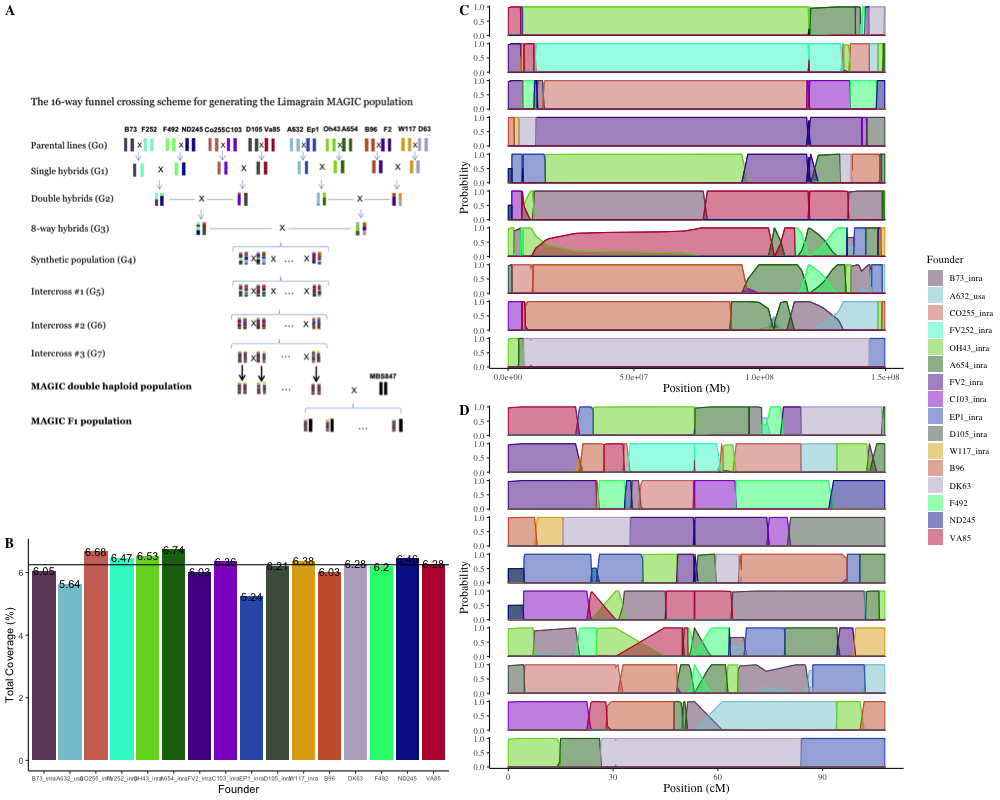
\includegraphics[width=\textwidth,height=14cm]{figures/Methods_Fig1.png}
\caption{\textbf{Structure, diversity, and founder representation of the MAGIC population}(\textbf{A}) The crossing scheme of the MAGIC population. (\textbf{B}) Total coverage of each founder across the population as a percentage. Black line shows expectation of equal distribution (6.25\%)  (\textbf{C}) Founder probabilities for 10 MAGIC DH lines on chromosome 10 in physical distance. (\textbf{D}) Founder probabilities for 10 MAGIC DH lines on chromosome 10 in genetic distance.}
\label{fig:figure1}
\end{figure*}

\subsection{Calculation of Identity-by-Descent and Haplotype Probabilities}
The identification of regions of shared genetic sequence between founder pairs would allow for the collapsing of founders into haplotypes.
IBD was measured from the 600K SNP data of the founders using the software RefinedIBD with a sliding window of 10 cM and a minimum IBD segment length of 0.2 cM \citep{Browning}.
The resulting segments of pairwise IBD between each of the 16 founders were used to identify distinct haplotype blocks.
We did this by moving along the chromsoome, starting a new haplotype block when a segment of pairwise IBD between founders started or ended.
Then, within blocks, we grouped all founders that were in IBD with one another into a haplotype.
Within blocks, the founder probabilities for founders within a haplotype were summed to obtain haplotype probabilities.
In certain instances, the pairs of founders that were in IBD with one another in a particualar haplotype block formed an incomplete graph, where  not all founders were in IBD with all other founders.
For the sake of simplicity, we continued with the assumption that all founders in a haplotype were in IBD with one another.
However, it is important to note that haplotypes called here do still possess genetic differences between founders, with some founders more different than others.
The haplotype probabilities were filtered for LD using an iterative approach where, for all haplotype blocks with the same number of distince haplotypes,a SNP was dropped if the correlation of probabilities between it and the kept SNP was greater than 0.95.
After filtering, a total of 11,105 sites were kept to represent haplotype blocks in the MAGIC DH lines.

\subsection{Association and QTL Mapping}
The R package GridLMM was used to run association mapping using the three different methods of representing the genotype data \citep{Runcie}.
The function GridLMM\_ML was used with the "ML" option.
The following three models were approximated by fitting each locus independently.
The three methods differed in the $X$ matrix used in the mixed linear model.
The model that encorporated the raw 600K SNP genotype data (hereafter referred to as $GWAS_{SNP}$) was:
\begin{equation}
\label{eqn:gridlmm1}
 Y = X_S{\beta_S} + Zu + \epsilon
\end{equation}

where $Y$ is the response variable, $X_S$ is an $n$ x $p$ genotype matrix with reference and alternate alleles represented as 0 and 1, respectively, $\beta_S$, is the effect size of the alternate allele, $Z$ is the design matrix, $u$ is the random effects of markers across the rest of the genome using the genomic relationship matrix, $K$, and $\epsilon$ is the error.GridLMM fit an $n$ x 1 matrix for each site $p$.

The model that encorporated the founder probabilities (hereafter referred to as $GWAS_F$) was:
\begin{equation}
\label{eqn:gridlmm2}
 Y = X_F{\beta_F} + Zu + \epsilon
\end{equation}
where $Y$ is the response variable, $X_F$ is a ($n$ x $p$) x $f$ matrix and $x_{fnp}$ is the probability that at site $p$, individuals $n$ was derived from founder $f$, $\beta_F$, is the effect size of each founder allele, $Z$ is the design matrix, $u$ is the random effects of markers across the rest of the genome using the genomic relationship matrix, $K$, and $\epsilon$ is the error. GridLMM fit an $n$ x $f$ matrix for each site $p$.
The model that encorporated the haplotype probabiliteis (hereafter referred to as $GWAS_H$) was:
\begin{equation}
\label{eqn:gridlmm3}
 Y = X_H{\beta_H} + Zu + \epsilon
\end{equation}
where $Y$ is the response variable, $X_H$ is a ($n$ x $p$) x $h$ matrix and $x_{hnp}$ is the probability that at site $p$, individuals $n$ has haplotype $h$, $\beta_H$, is the effect size of each haplotype allele, $Z$ is the design matrix, $u$ is the random effects of markers across the rest of the genome using the genomic relationship matrix, $K$, and $\epsilon$ is the error. GridLMM fit an $n$ x $h$ matrix for each site $p$.

 Significance cutoffs for p-values were obtained using permutation testing, taking the 5\% cutoff from 1000 permutations where genotypes were randomized relative to phenotypes for each method. Code for the analyses can be found [github link].
%We used the software GEMMA [reference] to build a mixed linear model to identify
% QTL due the faster run time of this software with larger datasets.


The support interval size response variable was represented both in terms of physical distance (Mb) and genetic distance (cM).
\subsection{Estimation of Effect Sizes}
We used the R package lme4qtl to calculate standard errors of effect sizes relative to the population mean (code provided) \cite{Ziyatdinov}.
For the $QTL_F$ method, probabilties were dropped (converted to NA) for individual founders at some sites if the sum of probabilities for a particular founder across all MAGIC lines was less than 1 or if there where fewer than 5 MAGIC lines that had a probability greater than 0.8 for one of the founders.
This same filtering was done with $QTL_H$ effect sizes for sites with low representation of particular haplotypes.
This was to ensure that effect sizes for individual founders and haplotype could be effectively estimated.
The comparison of effect sizes between methods was done using the effect sizes estimates of the most significant site within the QTL support interval.
For methods that did not identify a QTL detected in other methods, comparison of effect sizes used the site with the highest log10 p-value that overlapped with the QTL support interval from the method that did detect the QTL.
We confirmed that effect sizes calculated by GridLMM and lme4qtl matched one another, with the correlations in effect sizes between the two methods greater than 0.99.

\subsection{Method Comparison}
The results of the three methods of identifying QTL were compared using two main criteria: (i) presence or absence of identified QTL peaks and (ii) the size of QTL support intervals.
QTL support intervals were determined by identifying the most significant SNP for a QTL peak and demarcating the left and right bounds of the QTL as the left-most and right-most SNPs within a 100Mb window centered on the highest SNP that have a log10 p-value that is 2 log10 p-values below that of the highest SNP.
The detection of QTL was compared across the three methods for each phenotype.
A QTL was said to be identified across methods if the QTL support interval for that QTL overlapped between the three methods.
The effect of the method used on the size of QTL support intervals was investigated using the QTL which were identified by all three methods (n=40). The model constructed was:

\begin{equation}
\label{eqn:bounds}
 Support Interval Size = Environment_QTL + Method + \epsilon
\end{equation}

We also compared the individual QTL identified by the three models in regards to the percent of phenotype and genetic variance explained by the QTL, the minor allele frequency of the QTL in the population, and the standard errors of effect size estimates for the QTL. For each model, the highest non-significant peak within the support intervals of the QTL found in other models was used to represent the unidentified QTL. We tested for significant differences in these statistics between QTL that were identified or not identified in $GWAS_{SNP}$, $QTL_F$, and $QTL_H$.

We tested for differences between models in terms of the PVE by QTL that were detected or undetected. We fit a mixed linear model with the all combinations of method and whether or not a QTL was identified (i.e. $QTL_F$-True) as a fixed effects and individual QTL as random effects. We tested for significant differences between the least square means of the estimated fixed effects using a Tukey pairwise test.

\subsection{Tests for Epistasis}
We ran a genome scan for epsistatic interactions with \emph{vgt1}. The probability of the MAGIC lines having the MITE insertion at \emph{vgt1} was calculated by summing the founder probabilities for all founders that have the $MITE^+$ allele at the site closest to the location of the MITE in the B73 APGv4 assembly (list marker).
Lines that had uncertain allelic states at the MITE (0.05 > Pr(MITE) < 0.95) were dropped for the test.
We used a Bonferroni significance threshold adjusted for the number of tests.
We tested for epistasis using the 600K genotype data after filtering for LD (number of tests).

We also performed QTL mapping with $QTL_F$ using only the $MITE^+$ MAGIC.
This was to see if there were any other loci whose affect was only observed in the presence of the MITE.
Additionally, this provided an alternative was of testing for epistasis with \emph{vgt1} using the founder probabilities could not be fit with founder alleles there were not enough degrees of freedom to compare each founder.
We used the model from Equation \ref{eqn:gridlmm2} using DTA BLUP scores and each independent environment and the 5\% significance threshold for DTA.

\subsection{Test for Over- and Under-Representation of Alleles}
The rounded sum of the founder probabilities for each founder across all lines was used as an approximation of the number of lines that had that founder at a site.
This observed count was compared to a null expectation of $1\/16$ for equal distribution across lines (approximately 21 lines per founder).
We performed a $\rchi^2$ test for each site to determine if founder counts signficantly deviated from null expecation, adjusting for multiple testing (p-value<xx).
In order to ensure that significant $\rchi^2$ sites were not due to sequence similarities between founders, we performed the same test with haplotype probabilities (p-value<xx).
With haplotype probabilities, the null expectation was proportional to the number of founders grouped within each haplotype and the total number of unique haplotypes at the site.

\subsection{Flowering Time Enrichment Test}
We used a list of flowering time (FT) genes assembled by \citep{Li5} to test for enrichment of FT genes in haplotype $\rchi^2$ peaks.
Of the 907 genes, we used 88X which were aligned to chromosomes 1 through 10 in the B73 AGPv4 assembly \cite{Jiao}.
To determine a null distribution, we randomly sampled XX number of non-FT genes and counted the number that overlapped with regions within $\rchi^2$ peaks.
We compared this number to the actual number of FT genes that overlap with $\rchi^2$ peaks.

\subsection{Calculation of Flowering Time Polygenic Scores}
We calculated the polygenic scores (PGS) by summing DTA and DTS effect sizes across all sites.
To determine a null distribution of FT PGS, we also calculated PGS for 100 populations of simulated MAGIC lines.
We performed an X?? test to determine if the PGS of the actual DH lines were earlier than would be expected by chance.

%%%%%%%%%%%%%%%%%%%%%%%%%%%%%%%%%%%%%%%%%%%%%%%%%%%%%%
\section{Results}
%%%%%%%%%%%%%%%%%%%%%%%%%%%%%%%%%%%%%%%%%%%%%%%%%%%%%%
%Topic sentences

\subsection{MAGIC Population}

We developed a 16-parent MAGIC population using inbred lines representative of the diversity Flint and Dent heterotic groups of North America and Europe (Figure \ref{fig:figure1}A).
We genotyped 325 MAGIC DH lines from the population with 600K chips and measured 6 pheotypes across 6 environments from the MAGIC F1 lines, resulting from crossing the DH lines to an inbred tester, MBS847.
The distributions of the measured phenotypes were  approximately normal (Figure \ref{fig:supfigure1}).
Some deviations from the assumptions of normality were observed for days to silking (DTS) and, as a result, anthesis-silking interval (ASI).
Using the phenotype data from the six environments, we calculated BLUP scores for each of the MAGIC lines.

\subsection{Simulation and Validation of Founder Probabilities}

We partitioned the genomes of individual MAGIC lines into segments of ancestry from the 16 founders.
This allowed us to determine the predicted contribution of each founder to the population (Figure \ref{fig:figure1}B \& D).
The founder probabilities determined using R/qtl2 were able to assign founders to the actual MAGIC DH lines with high confidence (>0.90) for [percentage] of the 10 chromosomes of maize.
Our simulations suggest a very high ($\mu = 99.8\%, \sigma =0.011$) assignment accuracy (see methods).
This reinforced our confidence in the founder probabilties obtained from the actual data.

\subsection{Identity-By-Descent and MAGIC Haplotypes}
In some cases, the model which inferred founder identity in the MAGIC lines had high uncertainty, with probabilities split approximately equally between two founders.
We hypothesized that this uncertainty was due to the two founders having very similar genetic sequence at those regions, such that the model struggled to differentiate the two.
To assess the genetic similarity of the founders, we calculated Pairwise Identity-By-Descent (IBD) between all founders.
Areas of uncertainty in founder probabilities of the DH lines were associated with regions of IBD between two or more founder lines in that region of the chromosome (example figure).
The results showed that a total of [bp][cM] of genome were in IBD between at least two different founders.
The average size of an IBD segment between two founders was 140kb (0.51 cM) with a median of 122kb (0.46).

\begin{figure*}[ht]
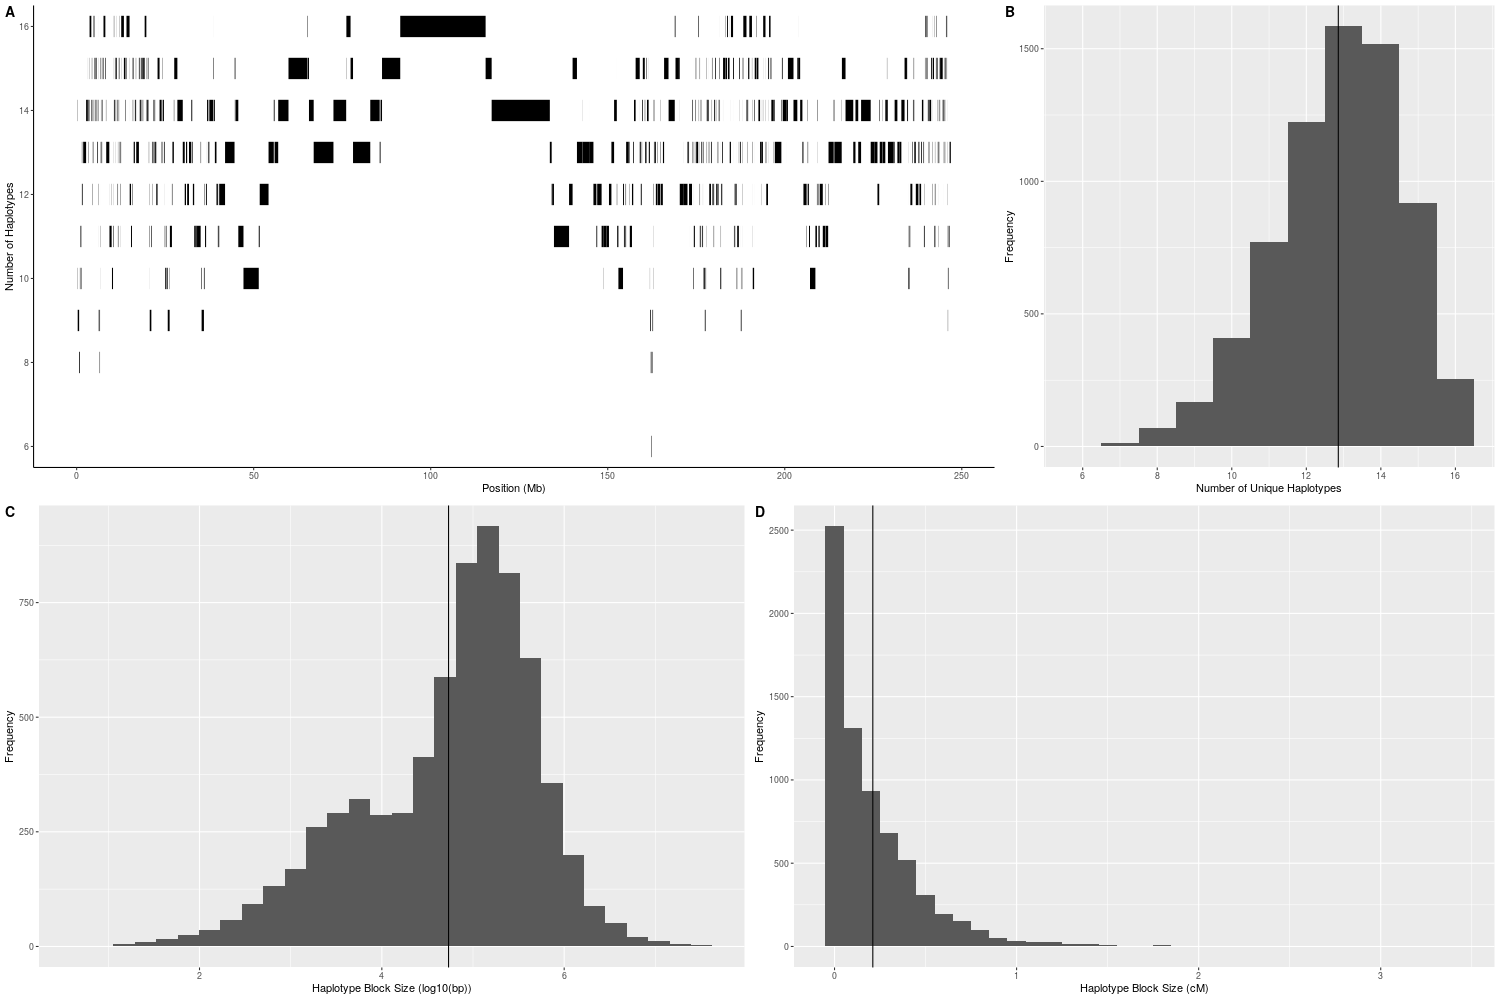
\includegraphics[width=\textwidth,height=10cm]{figures/figure2.png}
\caption{\textbf{Diversity and Size of Haplotype Blocks} The number of unique haplotypes among the 16 MAGIC founders across the 10 chromosomes of maize (\textbf{A}) The number of unique haplotypes per haplotype block and size of haplotype blocks along chromosome 4 in physical distance. (\textbf{B}) Distribution of unique haplotypes per haplotype block across the genome. (\textbf{C}) Distribution of haplotype block size in physical distance, represented as log10(bp). The black bar represents the average size. (\textbf{D}) Distribution of haplotype block size in genetic distance, represented as cM. The black bar represents the average size.}
\label{fig:figure2}
\end{figure*}

Pairwise IBD segments sizes ranged from 8 kb (0.3 cM) to  673 kb (1.61 cM).
For founder pairs that were found to be in IBD with one another, the total percentage of IBD between founders ranged from 0.0018\% (F492 and VA85) to 4.3858\% (B73 and A632), with an average of 0.06130\%.There were no IBD segments found for 18 of 120 possible pairwise founder combinations.
Amount of IBD between the founders and the tester, MBS847...
The Neighbor-Joining Tree of the relatedness of the 16 founders recapitulated the IBD results (Supplemental Figure). For a particular founder pair, B73 and A632, there were large segments where the lines shared haplotypes, and the tree placed them very close together.
This is consistent with pedigree of the lines, where A632 was derived from B14, a line from the same population as B73 (cite).
Due to the widespread Pairwise IBD between the founders, it appeared that many founders shared haplotypes
Within individual blocks of ancestry, we collapsed founder alleles that were identical by descent into a single haplotype.
The number of unique haplotypes within haplotype blocks varied across chromosomes, ranging 6 at the lowest to 16 at the highest (Figure  \ref{fig:figure2}A & B). The average number of unique haplotypes per haplotype block was 13 ($\mu = 12.85, \sigma =1.71$) (Figure \ref{fig:figure2}B).
The a wide range of haplotype block sizes with the average physical size of haplotype blocks being 303.7 kb ($\sigma =1.71$Mb) (Figure \ref{fig:figure2}C)).
The largest haplotype block was 39.3 Mb long on chromosome 7, which had 16 unique haplotypes.
In genetic distance, haplotype block sizes range from 0 to 3.4 cM, with an average of X (Figure \ref{fig:figure2}D).

\begin{figure*}[ht!]
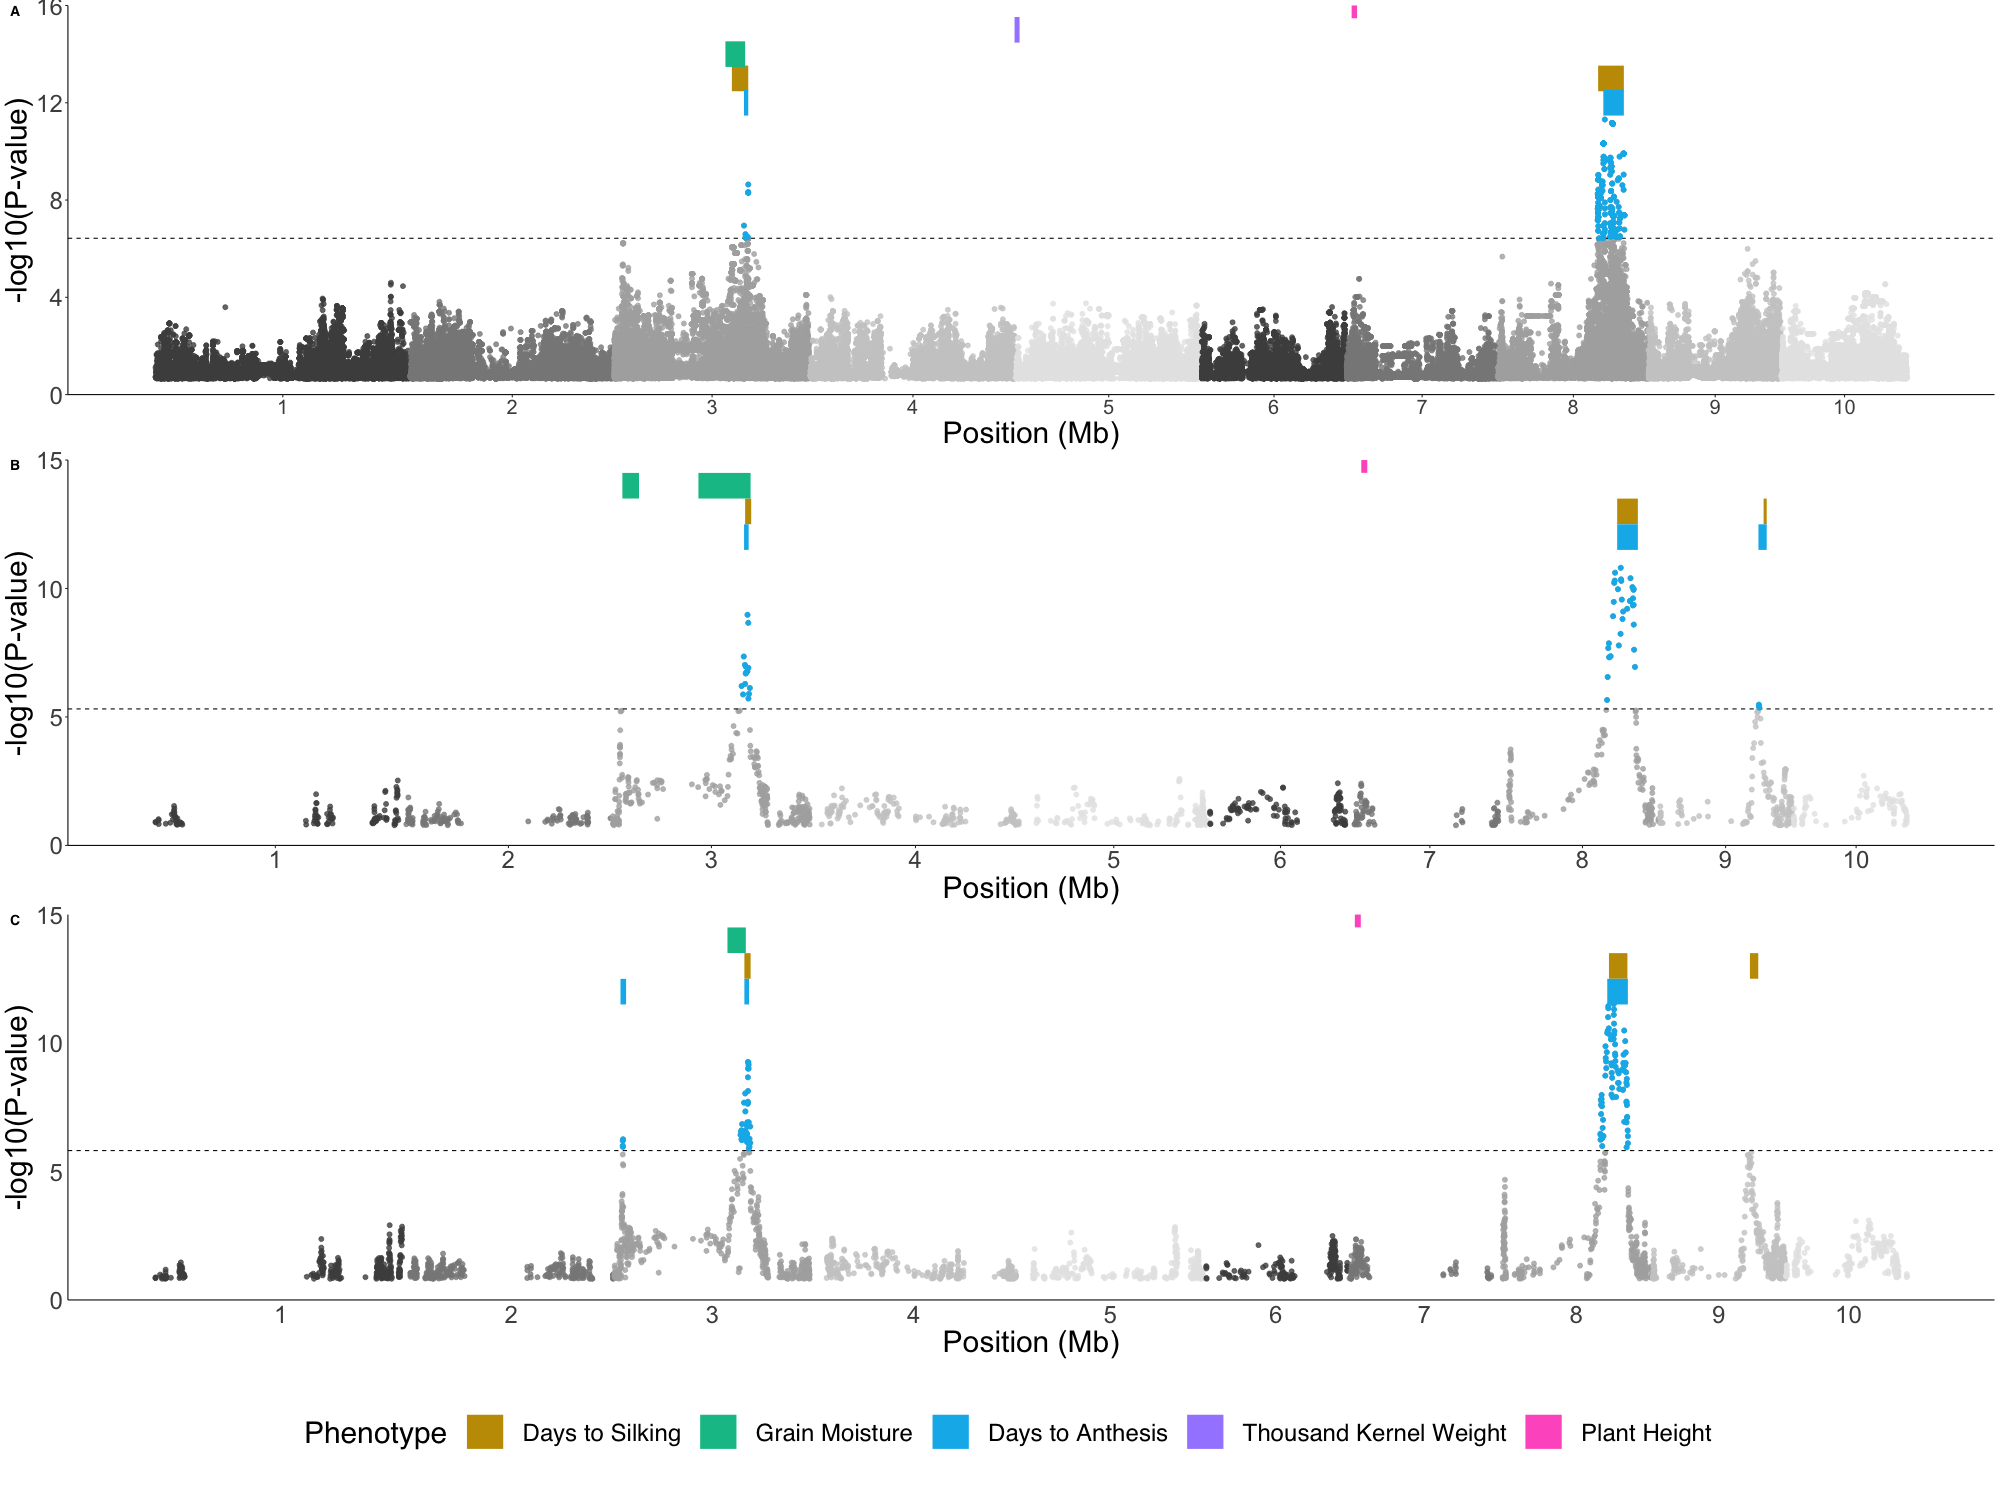
\includegraphics[width=\textwidth,height=14cm]{figures/Methods_Fig3_alltraits.png}
\caption{\textbf{Results of three methods of QTL identification} Colored points represent significant QTL for Days to anthesis (DTA) BLUPs above the 5\% significance threshold from 1000 random permutations. Colored bars represent the location QTL support intervals for five other BLUP phenotypes (list colors and add legend, make the small intervals more visable) \textbf{top} GWAS results using the 600K SNP array. \textbf{middle} Results from QTL mapping using founder probabilities \textbf{bottom} Results from QTL mapping using haplotype probabilities}
\label{fig:figure3}
\end{figure*}


\subsection{QTL Mapping and Association Mapping}
We performed association mapping using three models of the allelic state of qtl2.
The first method, $GWAS_{SNP}$, used SNP genotypes obtained from the 600K chip, assuming that QTL are bi-allelic.
The second method, $QTL_F$, used probabilities of founder identity in chromosome segments, assuming that a QTL had as many alleles as founders.
The second method, $QTL_H$, used probabilities of haplotype identity in chromosome segments, assuming that a QTL had as many alleles as ancestral haplotypes.
The three methods varied in their ability to identify QTL.
Figure \ref{fig:figure3} shows the Manhattan plots from the three methods for BLUP DTA overlayed with the support intervals of significant QTL for all BLUP phenotypes.
For DTA, all three methods easily identify two large QTLs, \emph{qDTA3\_2} on chromosome 3 and \emph{qDTA8} on chromosome 8. These QTL correspond to three previously identified QTL, \emph{vgt3} for \emph{qDTA3\_2} and \emph{vgt1} and \emph{vgt2} for \emph{qDTA8}.
In addition, there are multiple QTL that are found by only a subset of the models.
Using BLUPs, the $GWAS_{SNP}$ method was able to identify one QTL on chromosome 5 for thousand-kernel weight, \emph{qTKW\_5} that was not found in either $QTL_F$ or $QTL_H$.
A second QTL on chromosome 3 for DTA, \emph{qDTA3\_1}, was only found with the $QTL_H$ method.
A DTA QTL on chromosome 9, \emph{qDTA9} and a harvest grain moisture QTL on chromosome 3, \emph{qHGM3\_1} were only found using $QTL_F$.
However, a QTL for DTS with overlapping support intervals to \emph{qDTA9} was found in both $QTL_F$ and $QTL_H$.

We performed QTL mapping separately in each of the 36 environment:phenotype combinations, plus the across-environment averages of the 6 traits, for a total of 42 separate analyses.
When we called each environment-phenotype as its own trait (i.e days to anthesis in Blois, 2014), a total of 46 unique QTL were identified from all three mapping methods.
26 (57\%) QTL were identified by all three models.
6 QTL were found in both $GWAS_F$ and $GWAS_H$ and 1 QTL was found in both $GWAS_{SNP}$ and $QTL_F$.
7, 3, and 3 QTL were found in only $GWAS_{SNP}$, only $QTL_F$, and only $QTL_H$, respectively (\ref{fig:supfigure2}).

Next we merged QTL of the same phenotype from different environment based on overlapping support intervals.
There were 20 unique across-environment QTL identified from all methods.
10 (50\%) of these across-environment QTL were found in more than one environment.
12 across-environment QTL were found using BLUPs and 2 of these QTL were not found in any individual environment.
6 (0 unique) QTL were found in Blois, 2014, 7 (1 unique) in Blois, 2017, 7 (3 unique) in Graneros, 2015, 5 (1 unique) in Nerac, 2016, 6 (3) in St.Paul, 2017, and 3 (0 unique) in Szeged, 2017.

Despite differences in the models, the power to identify and refine the location of QTL was similar across the three methods.
Overall,differences between the three approaches were relatively subtle.
$QTL_F$ was able to identify the most QTL, regardless of changes in the significance threshold (Supplemental Figure).
Individual QTL that were found in one method at the 5\% significance threshold usually became significant in other methods when at the 10\% threshold, indicating that the differences in the ability to detect these QTL between methods is mostly due to difference in power (\ref{fig:supfigure3}).
Nonetheless, there were multiple QTL that were identified in only one method. There were 10 QTL that appeared in one method and not in any others, mostly related to grain yield and thousand kernel weight traits.

There was no significant different in the size of QTL support intervals between methods, both in physical (F-value = 0.5157, p-value = 0.5989) and genetic distance (F-value = 1.1658, p-value = 0.3165).
Although on average, the physical and genetic size of $GWAS_{SNP}$ support intervals were larger than those of $QTL_F$ and $QTL_H$ support intervals, the difference was not significant and was most likely due to a few outliers.
The average physical sizes of QTL bounds were 14.4 Mb (SE = 1.18 Mb) for $GWAS_{SNP}$, 12.8 Mb (SE = 1.07 Mb) for $QTL_F$, and 13.4 Mb (SE = 1.09 Mb) for $QTL_H$.
The average genetic sizes of support intervals were 6.24 cM (SE = 0.353 cM) for $GWAS_{SNP}$, 5.85 cM (SE = 0.320 cM) for $QTL_F$, and 5.51 cM (SE = 0.325 cM) for $QTL_H$.


\begin{figure}[ht]
\centering
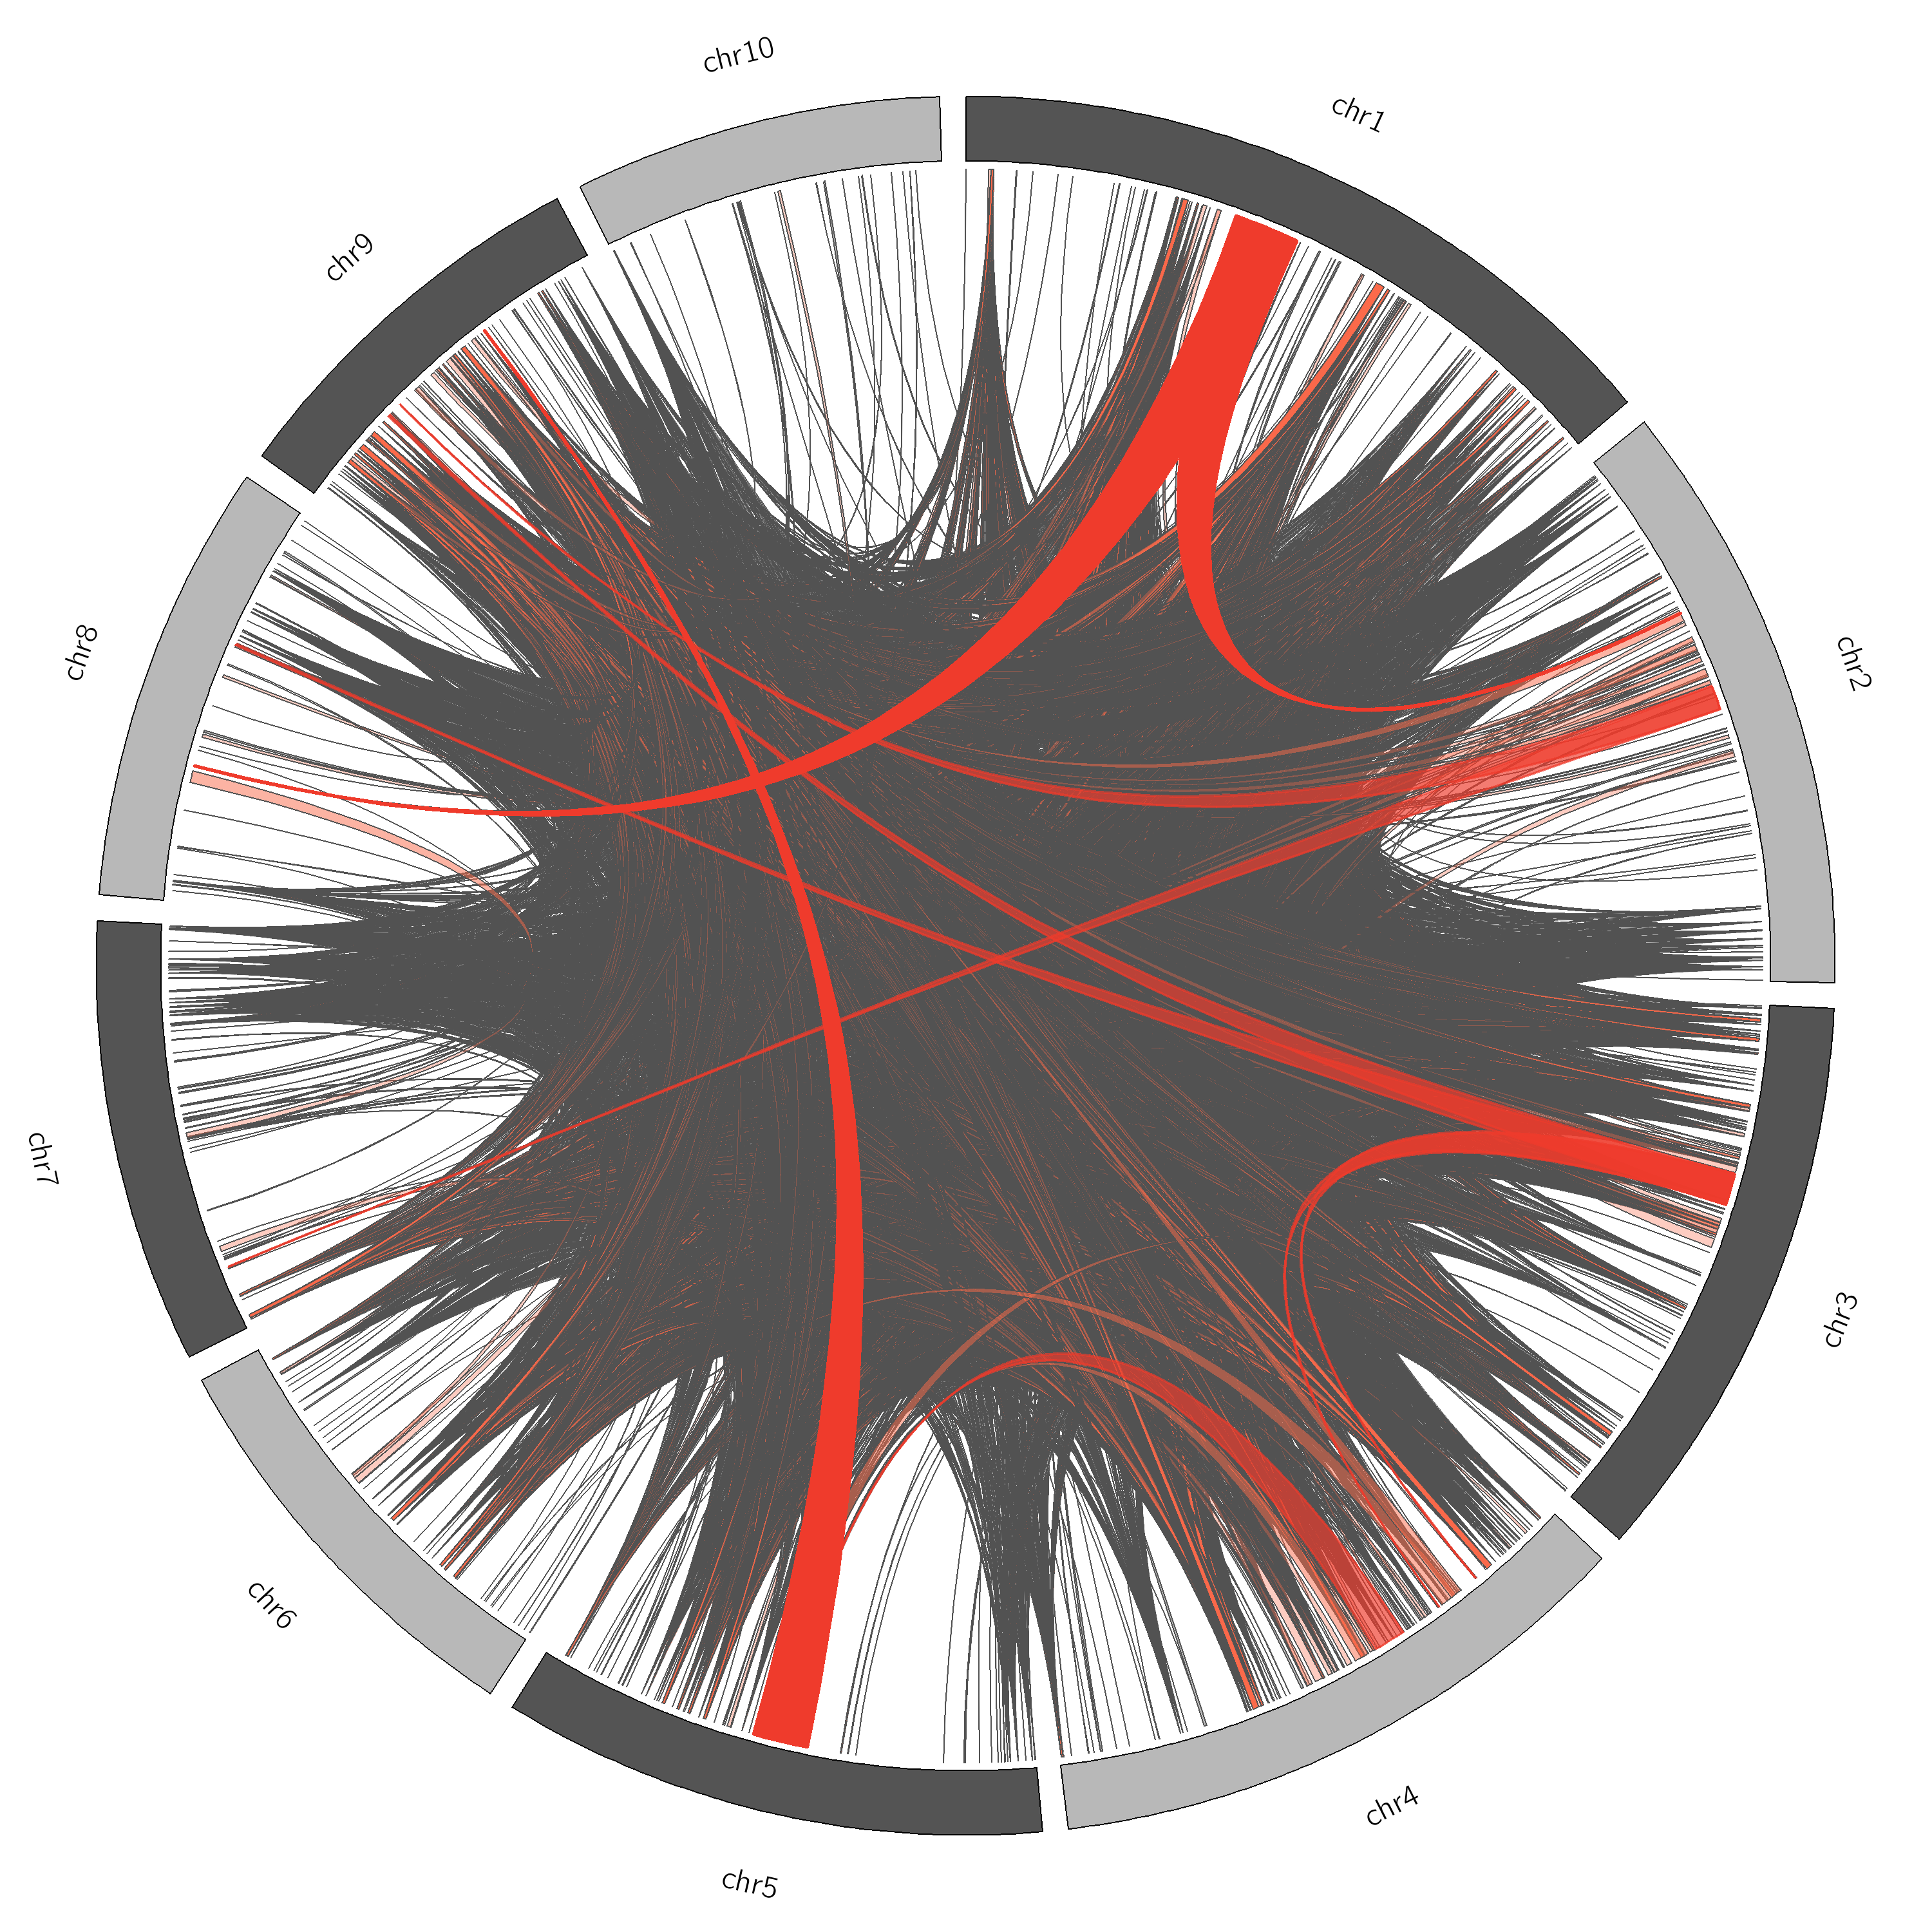
\includegraphics[width=\linewidth]{figures/circos.png}
\caption{\textbf{Interchromosomal Linkage Disequilibrium in the MAGIC Population} Ribbons represent regions of $R^2$ > 0.8 between consecutive SNPs on different chromosomes. Dark, solid, red bands are regions larger than 20Mb on at least on of the chromosomes. Lighter, translucent red bands are regions greater than 1Mb and less than 20Mb. Grey bands are regions larger than 10kb.}
\label{fig:circosfigure}
\end{figure}

\subsection{Variation in Effect Sizes}
In select cases, effect sizes and allelic state of QTL seemed to explain the models' differing success in detection.
Even for QTL that were identified by all methods, the estimated effect sizes of the QTL differed both across environments and between methods (include figure).
For QTL that were found with some methods and not others, we attempted to examine the effect sizes to see if they provided insight into the genetic architecture of the QTL.
%This might suggest some mechanism besides differences in statistical power that would explain the differences in QTL detection ability.
%Looking at the effect sizes of the most significant SNPs within QTL support intervals, the effect size of the founders with the alternate allele are different than the single effect size of the alternate SNP allele provided by $GWAS_{SNP}$.
%For QTL that were found with both $GWAS_{SNP}$ and $QTL_F$, the effect sizes match up relatively better, but still show significant differences.
%Looking at the founder effect sizes of the most significant site from the $QTL_F$ within the $GWAS_{SNP}$ QTL support interval, the effect sizes have larger standard errors [figure/stats??].

%In most cases, the effect sizes of haplotypes average out the effect sizes of founders that are grouped together, weighted by the frequency of the founders in the MAGIC lines [stats??].
For QTL detected in $QTL_F$ and not $QTL_H$, generally, there were higher numbers unqiue of haplotypes in these cases [stats].
Comparing effect sizes of QTL that were identified in $QTL_H$ and not $QTL_F$, there tended to be fewer unique haplotypes at these QTL regions and the effect sizes of haplotypes that grouped together more than one founder were similiar to the estimated effect sizes of those founders [stats?? figures?].

For each model, we compared QTL detected by that model to those not detected (see Methods).
Comparing within models, we found that there were significant differences in the proportion of phenotypic variance explained (PVE) by QTL that were and were not detected by individual models (Figure \ref{fig:pvefigure}).
Perhaps unsurprisingly, the PVE of detected QTL were signfiicantly higher than that of undetected QTL for $QTL_F$ (t-ratio -4.566, p-value 0.0002) and  $QTL_H$ (t-ratio -4.145, p-value 0.0009).
However, QTL not detected by $GWAS_{SNP}$ had signficantly higher PVE than those detected by that method (t-ratio 3.267, p-value 0.0178).
Between models, QTL detected by $QTL_F$ and $QTL_H$ explained significantly more phenotypic variance than those detected by $GWAS_SNP$ (t-ratio -28.883 p-value <.0001; t-ratio -31.278 p-value <.0001), although there was no significant difference between $QTL_F$ and $QTL_H$ (t-ratio 1.658, p-value 0.5629)

\begin{figure}[ht]
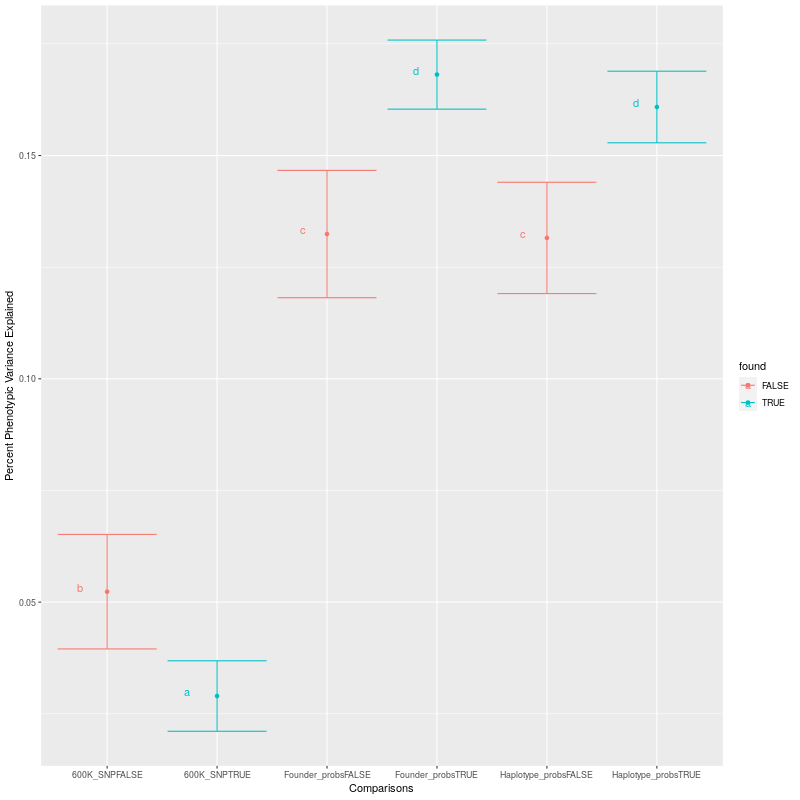
\includegraphics[width=\linewidth]{figures/pve_contrasts.png}
\caption{\textbf{Percent Phenotypic Variance Explained By Detected and Undetected QTL Between Methods} Color indiciates whether or not QTL were detected in that group. Letters represent significantly difference groups from a Tukey pairwise test.}
\label{fig:pvefigure}
\end{figure}

\subsection{Variation around \emph{vgt1} and \emph{vgt2}}
One notable QTL that was identified by all three models using BLUPs (Figure \ref{fig:figure3}) and nearly all individual environments was qDTA8, a large QTL on chromosome 8 that was strongly correlated with variation in days to anthesis, as well as days to silking.
The support interval for this QTL overlapped with two previously characterized flowering time QTL, \emph{vgt1} and \emph{vgt2}.
These known flowering time loci provided a useful benchmark for comparison of these approaches.

At \emph{vgt1}, the founders are segregating ($MITE^+$/$MITE^-$) for the causal variant, a MITE insertion in a conserved non-coding sequence upstream of \emph{ZmRap2.7} (\cite{Salvi}; \cite{Castelletti}).
Looking at the most significant SNP for \emph{qDTA8} from $GWAS_{SNP}$, the alternate allele correlated strongly but imperfectly with the presence of the MITE in the founders (correlation).
We expected to see $QTL_F$ effect sizes at this locus that match the allelic state of the founders, with $MITE^+$ founders having earlier effect sizes and $MITE^-$ founders having later effect sizes.
However, for some founders the $QTL_F$ effect sizes at \emph{vgt1} deviated from those expections (Figure \ref{fig:foundervgt1figure}).
Four $MITE^+$ founders, A632, F252, C103, and F492, had DTA BLUP effect size estimates later than the population average.
While only one founder, F252 had a 95\% confidence interval not overlapping zero, all of them had effect sizes significantly later than the other $MITE^+$ founders (pvalue).
This pattern was also seen in the effect sizes estimated in individual environments (Supplemental figure).
Lastly, at the most significant hit from $QTL_H$, founders are grouped into haplotypes consistent with their allele at the MITE, but there are still far more than 2 distinct haplotypes (12?).
Analysis of the haplotype structure in the region around \emph{vgt1} in the 16 founders showed clear differences between those that did and did not have the MITE insertion, but did not differentiate $MITE^+$ late founders from $MITE^+$ early founders (supplemental figure).

These results suggested to use that there may be an epistatic interaction between \emph{vgt1} and the genetic background.
A genome scan for epistasis between \emph{vgt1} and other loci did not yield any significant interactions.
However, $QTL_F$ using only MAGIC lines predicted to have the MITE had two significant DTA BLUP QTL in the region of \emph{vgt1} (figure).
One of these significant sites is located in close proximity to the causal gene for \emph{vgt2}, \emph{ZCN8}, and is mostly explained by this linked QTL.
However, the second significant site is located ~15Mb downstream of \emph{vgt1}, suggesting that some local variation around the region of \emph{vgt1} impacts the affect of the QTL on flowering time.

% Look at variants around ZCN8

% Look at variants around ZMMADS69 (do we know causal variants?)

\begin{figure}[ht]
\centering
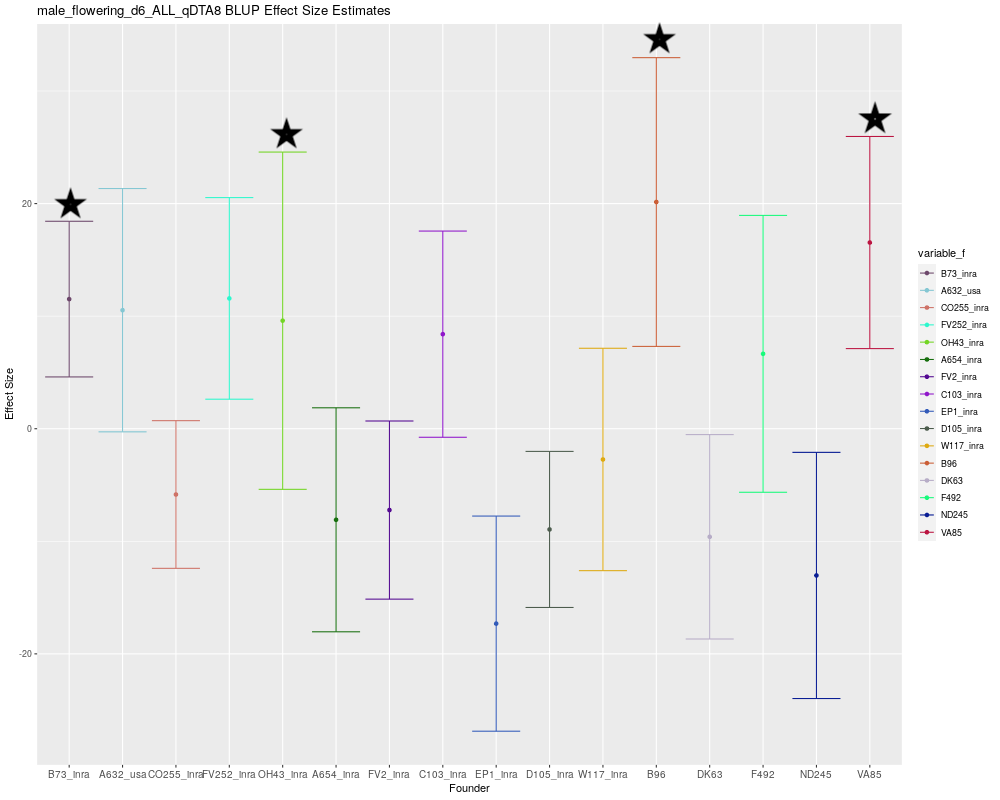
\includegraphics[width=\linewidth]{figures/male_flowering_d6_ALL_qDTA8_BLUP_founder_effect_sizes_lme4qtl.png}
\caption{\textbf{Estimated founder effect sizes for qDTA8} Estimates of founder effect sizes centered around the population mean for Days to Anthesis (DTA) BLUP phenotypes using $QTL_F$. Positive effect sizes indicate later flowering and negative effect sizes indicate earlier flowering. [Stars indicate founders that do not possess the MITE insertion ($MITE^-$)]}
\label{fig:foundervgt1figure}
\end{figure}

\subsection{Founder Representation and Linkage Disequilibrium}

The MAGIC population showed an overall balance of coverage from the 16 founders (Figure \ref{fig:figure1}B).
Analysis of the MAGIC population showed that the overall representation of the 16 founders in the MAGIC DH lines was relatively even, with the highest percentage founder, A654, representing 6.741\% and the lowest percentage founder, EP1, representing 5.237\%.
However, multiple chromosome regions deviated significantly from the expected equal distribution.
Across individual regions of each chromosomes, 33\% of founder probability sites significantly deviated from null expectations ($\rchi^2$ test p-value < 6.82e-07 (15 df)) (Supplemental Figure).
The same $\rchi^2$ test performed on 100 simulated MAGIC populations of 325 individuals resulted in only 4 significant $\rchi^2$ peaks, showing that the over- and under-representation of certain founder alleles was greater than would be expected by chance.
One potential reasons for this observation was that the HMM in R/qtl2 was confusing founders that were in IBD with one another.
In order to ensure that these chi-squared peaks were not a result of technical error, we performed the same chi-squared test using haplotypes rather than founders.
Using haplotype probabilities, XX\% of sites deviated from null expectations...
Together, these results suggests that the over- and under-representation of founder alleles in the MAGIC population is biological, rather than a result of model error, and perhaps evidence of selection for or against particular founder alleles.

We estimated recombination rates and linkage disequilibrium across the MAGIC lines.
The founder probabilities showed levels of recombination in the MAGIC population that are consistent with expectations from the simulated MAGIC populations [I need to figure this out].
The intra-chromosomal LD structure show LD breakdown consistent with many recombination events.
The average linkage disequilibrium $R^2$ 50 for the population was XX.
Unexpectedly, there was a large amount of high inter-chromosomal LD (\ref{fig:circosfigure}).
Of a total of 9,796,630 SNP pairs with an $R^2$ greater than or equal to 0.9, 365,345 (3.7\%) of those pairs came from different chromosomes.
The number and size of inter-chromosomal high LD regions were more than would be expected by chance. In 100 simulated populations, there were no SNP pairs with $R^2$ greater than 0.9 detected between chromosomes.
Interestingly, a large segment of interchromosomal-LD between chromosome 3 and chromosome 8 (\ref{fig:circosfigure}) overlaps with the support intervals for \emph{qDTA8} and \emph{qDTA3-2}, corresponding to \emph{vgt1}\\ \emph{vgt2} and \emph{vgt3}, respectively.

% Selection on flowering time
\subsection{Evidence of Selecion on Flowering Time}
We had reason to believe that selection on flowering time occurred during the making of the MAGIC population.
When MAGIC DH lines were crossed to the inbred tester to produce MAGIC F1s, the DH lines needed to nick with the tester in order for crosses to be made.
The tester, MBS847, is a generally later flowering line is $MITE^-$ at \emph{vgt1} \cite{Chardon}.
For this reason, we would expect that, if selection on flowering time had occurred, most of the genetic variation that was selected against would have been for earlier flowering alleles.
We tested to see if genes involved in flowering were enriched in $\rchi^2$ peaks, where some founderss and haplotypes were significantly over- or under-represented.
However, the number of FT genes found within $\rchi^2$ peaks was not significantly different than were expected by chance (\ref{fig:supfigure4}).
%Presence/absence of FT genes
Therefore, there is no evidence that the over- and under-representation of particular founders and haplotypes was due to the presence of flowering time genes within these regions.

Due to the fact that MBS847 is earlier flowering, we would expect that earlier flowering alleles would be selected against and be at a lower frequency in the resulting MAGIC F1s.
The polygenic score (PGS) for DTA and DTS for the lines from the 100 simulated MAGIC populations were .. compared to the observed PGS of the actual MAGIC lines.

%Add legend to figure

%%%%%%%%%%%%%%%%%%%%%%%%%%%%%%%%%%%%%%%%%%%%%%%%%%%%%%
\section{Discussion}
%%%%%%%%%%%%%%%%%%%%%%%%%%%%%%%%%%%%%%%%%%%%%%%%%%%%%%

We used three models of QTL allelic states to identify QTL in the MAGIC population, a bi-allelic model ($GWAS_SNP$), a founder multi-allelic model ($QTL_F$), and an ancestral haplotype mult-allelic model ($QTL_H$).
The $GWAS_{SNP}$ method should be most powerful at identifying QTL for which the causal variant is biallelic and the tagged SNP is in tight LD with the causal variant.
However, for multi-allelic QTL or QTL for which LD is low between tagged SNPs, this method should have lower power.
$QTL_F$, which assumes that all founders possess distinct alleles, increases the odds of detecting both QTL that are multi-allelic and QTL whose causal variant is not in tight LD with any one tagged SNP.
The higher number of parameters that must be fit by this model may also reduce power.
Lastly, $QTL_H$ potentially improves on the power of $QTL_F$ to detect QTL that meet the above criteria by reducing the number of parameters that must be estimated.
There is, however, the potential for $QTL_H$ to obscure the signal of some QTL if founders are called as being in IBD with one another when they actually differ for the causal variant.
Due to the fact that $QTL_H$ and $QTL_F$ take into account recent recombination events, whereas $GWAS_{SNP}$ uses historical recombination, we predicted that founder and haplotype mapping would result in higher resolution of QTL support intervals. Higher resolution QTL are ideal in that they makes it easier to narrow down candidate genes and potential causal variants when the support interval is smaller.


The results of using the three models of genetic architecture to identify QTL suggest that each has its own advantages and disadvantages in terms of how many and which QTL they can identify.
Overall, the $QTL_F$ performed the best in terms of the number of QTL identified, although there were multiple QTL identified uniquely in all models.
We conclude that if the goal of a study is to find as many QTL as possible, than it would be most useful to employ all three models to maximize QTL identification.
The lack of significant difference in the genetic size of support intervals for the QTL found in the three methods suggests that the differences in QTL detection ability are more a result of differences in statistical power than a difference in ability to account for recombination events.

Previous studies have compared similar models in different maize populations and using different methods of calculating haplotype blocks between parents (\cite{Leroux} and \cite{Giraud} \cite{Garin}).
Interestingly, the performance of the three models differs across studies. \cite{Giraud} found that their haplotype model outperformed the founder and SNP models in terms of the number of QTL identified using EU-NAM Flint and Dent maize populations. In contrast, \cite{Garin2} found that in the EU-NAM Flint population, the bi-allelic model detected a larger number of unique QTL, compared to parental or ancestral haplotype models.

The performance of the three models seems to depend heavily on the diversity of the parents used to generate the population.
For populations with more diverse founders, it would be expected that there would be fewer shared haplotypes between founders, reducing the efficacy of a haplotype model \cite{Giraud}.
The fact that the $QTL_F$ model outperformed the $QTL_H$ and $GWAS_{SNP}$ in this population suggests that the MAGIC population contains a relatively more diverse representation of European and North American flint and dent than populations used in previous studies.
It is also possible that the structure of multi-parent populations has an effect on the performance of the three models, compared to previous studies which used nested association mapping (\cite{Giraud}; \cite{Garin2}) and and diallel populations \cite{Bardol}.

Differences in the estimated effect sizes across models offer suggestions as to the reason for their differences in QTL detection.
%The differences between $GWAS_{SNP}$ and $QTL_F$ may be due to the fact that the most significant SNP in $GWAS_{SNP}$ and the most significant site in $QTL_F$ may be different regions with slightly different LD structure.
QTL that were only found in the $GWAS_{SNP}$ method most likely have a bi-allelic causal variant.
It is likely that the increased number of parameters in the $QTL_F$ and $QTL_H$ models reduce statistical power when the true number of functional alleles is low.
Multi-allelic QTL were more likely to be identifed by the $QTL_F$ or $QTL_H$ models and not the $GWAS_{SNP}$ method unless the effect size was large.
For QTL that were not identified by  the $QTL_H$ method, particularly for QTL that were successfully identified by $QTL_F$, the most likely reason is a failure of $QTL_H$ to accurately represent the true haplotype structure of the QTL region.

The $QTL_H$ method's assumption that founders share ancestral haplotype varied in its ability to improve QTL detection.
For QTL that were identified in the $QTL_H$ method and not the $QTL_F$ method, the lower number of unique haplotypes suggests that $QTL_H$ was more successful in finding these QTL due to improved power when there were fewer functional alleles than founders.
The lack of significant improvement of the $QTL_H$ method relative to the others in some cases is most likely the result of the formation of haplotypes based off of sequence information that do not accurately reflect the functional haplotypes of the founder for particular phenotypes.
Grouping of two or more founders into the same haplotype that do not share the same functional alleles underlying a QTL would result in a decrease in the ability to accurately estimate haplotype effect sizes and a reduction in signal.

It should also be noted that in the process of calculating pairwise IBD and assigning founders to haplotypes requires an inherently arbitrary significance threshold for calling founders as in IBD or not.
In our case, this resulted in some incomplete haplotype graphs, meaning that in some cases, most, but not all founders grouped into the same haplotype were in pairwise IBD with the other founders in the haplotype.
On the whole, most QTL were found by all three methods, so there was limited abiity to draw reliable conclusions about underlying mechanisms that caused the methods to perform better or worse.
Generally, the comparison of QTL detection and effect size estimates suggested that the methods failed and succeeded on a QTL-by-QTL basis.
This is to be expected, as each QTL is the result of a distinct causal variant with a different number of alleles within the population.
Whether QTL that appeared in only one method are due to false positives or true differences in the methods' abilities to identify QTL with different genetic architectures cannot be determined.

Many of the QTL identified in the MAGIC have underlying candidate genes or have been found in previous studies, providing support to their biological reality .
Multiple flowering time QTL support intervals overlap or are close by previously identifed flowering time genes and QTL.
\emph{qDTA9} is nearby the previously identified maize flowering time gene \emph{ZmCCT9} \cite{Huang3}.
\emph{qDTA3-2} overlaps with \emph{Vgt3}, whose underlying gene was identified as \emph{ZmMADS69} \cite{Liang}.
\emph{qDTA3-1} is nearby a recently identified flowering time QTL also associated with phasphatidylcholine levels \cite{RodriguezZapata}.
The support interval for \emph{qDTA8} overlaps with two flowering time QTL, \emph{vgt1}, which we discuss in length, and another, \emph{vgt2}. The causal gene for this QTL is \emph{ZCN8}, which is the maize ortholog of FT in \emph{Arabidopsis} \cite{Lazakis}.
Variation in the promoter region of \emph{ZCN8} between temperate maize and teosinte suggests that earlier flowering alleles were under selection during the precess of maize domestication \citep{Guo};\citep{Bouchet}.
Overlap of other QTL with previously identified QTL...
It is interesting to note that there is strong overlap in the support intervals of QTL found on chromosome three between flowering time and harvets grain moisture (Figure \ref{figure3}), perhaps due to developmental pleiotropy linking flowering time and the moisture of kernels at harvest.

The MAGIC population presented here provides a useful resource for investigating quantitative trait variation in temperate maize.
As a multi-parent population, it has the advantages of increased diversity compared to bi-parental mapping populations, no population structure , and higher power to detect QTL with lower allele freqeuencies.
In contrast, it's disadvantages include lower power for detecting epistasis. In addition, Although theoretically the design should result in equal distribution of parents, this does not always appear to be the case.
The complex crossing scheme has the potential to introduce the influence of selection.
Purifying selection may actually reduce the genetic variation that we are attempting to study.

Simulations of the MAGIC population provide an opportunity to validate assignment of founder identities, as well as generate null expectations for various aspects of the population.
We made our own package due to the complicated nature of the crossing scheme.

The population displayed unexpected patterns of inter-chromosomal LD and uneven founder representation.
High over- or under-representation of some founder alleles may be due to these founders being in close IBD with another founder, resulting in uncertainty in the founder probablities.
Another possible explanation is that there was selection against these founders during the breeding process.
The high levels of inter-chromosomal LD detected in the MAGIC population deviates significantly from null expectations obtained from simulations.
If we assume that the simulated populations are accurate representations of the construction of the MAGIC population without selection, this result would suggest that the differences in founder representation observed in the actual population may be due to selection for or against certain founder alleles.

Another interesting observation of the population was the relatively high levels of inter-chromosomal LD, which deviated significantly from that obtained from simulations.
Inter-chromosomal LD has been detected in multiple populations of domesticated organisms, where breeding has resulted in the preservation of certain combinations of favorable alleles between chromosomes \cite{Robbins} \cite{MalyshevaOtto}.
Strong selection and positive or negative epistasis in natural populations have also been shown to create a pattern of interchromosomal LD (\cite{Kulminski} \cite{Gupta} \cite{Hench} \cite{Petkov}).
Both of these results suggest that forces other than those of random segregation have operated on the MAGIC population.
Another potential consequence of inter-chromosomal LD is the chance for confounding of association analyses, namely resulting in the detection of "ghost" QTL.
Although for the discussed QTL detected that were in LD with one another, \emph{qDTA8} and \emph{qDTA3-2}, their effects on flowering time were independent, the chance for false positives and innacurate support intervals due to LD structure is still worth noting.

There was reason to suspect that there had been purifying selection on flowering time over the course of the creation of the MAGIC population.
However, there was no enrichment of flowering time genes in regions where some founders were more or less represented than expected by chance.
Polgenic scores of flowering time compared to simulations...

Due to the fact that it is segregating for \emph{vgt1}, this population provides an opportunity to further study the mechanism behind the QTL's affect on flowering time.
%Deviation from expectations in the founder effect sizes could be due to interaction with local genetic background or differences in estimation error due to lower representation of certain founders in the MAGIC lines at this region.
One benefit of using founder and haplotype approaches lies in the potential to dissect the effects of individuals founders and/or haplotypes within QTL.
This allowed us to look more closely at a well-characterized, large effect flowering time QTL, \emph{vgt1} and observe an interesting pattern of effect sizes that deviated from our expectations based on previous research.
The results of $MITE^+$ $QTL_F$ are consistent with previous research that showed that local genomic differences around \emph{vgt1} affect allelic effects in an admixed population of Flint and Dent lines (\cite{Rio}).
This opens up new areas of inquiry for future studies.


\section{Conclusion}

%\subsection{another figure}
%This is a full size figure (Figure \ref{fig:S1}) just add stars to the figure


\section{Acknowledgments}
We would like to acknowledge Limagrain for the use of their data and their feedback and support that made this work possible.

\bibliography{magic_tex}

%\pagebreak
\onecolumn
\beginsupplement
\section*{Supplement}
\begin{figure}[ht]
\centering
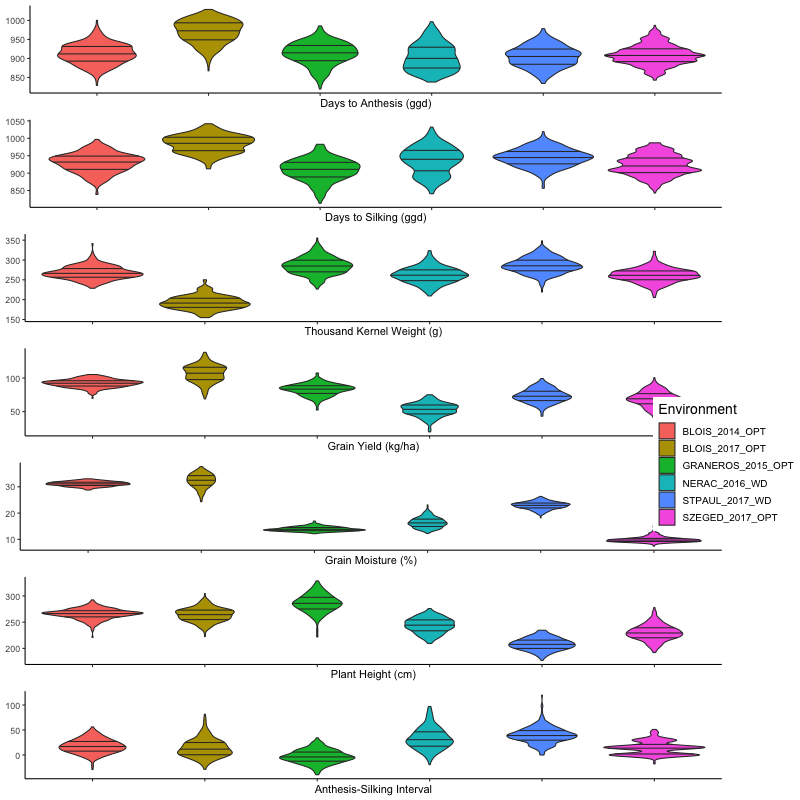
\includegraphics[width=\linewidth]{figures/Methods_Fig2_violinplot.png}
\caption{\textbf{Distribution of phenotypes} The density plots of the six measured phenotypes. The vertical bar represents the mean, and the grey shading shows two standard deviations. The heritability of each trait is shown on the right.}
\label{fig:supfigure1}
\end{figure}

\begin{figure}[ht]
\centering
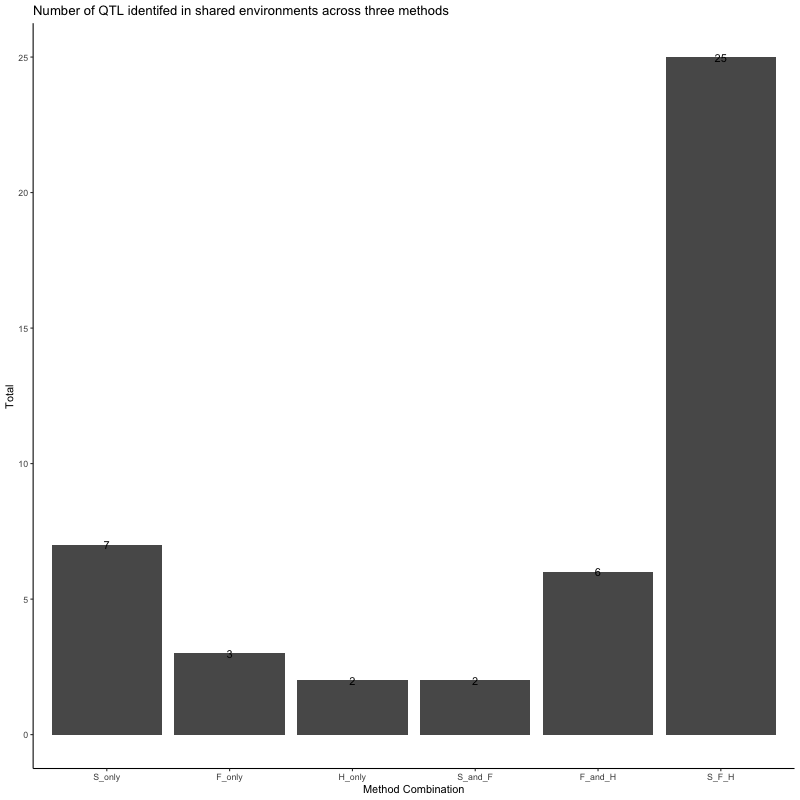
\includegraphics[width=\textwidth,height=14cm]{figures/environment_QTL_by_method.png}
\caption{\textbf{Number of Environment-Specific QTL Found by Method} S: $GWAS_{SNP}$, F: $QTL_F$, H: $QTL_H$. Environment-specific QTL are QTL for a phenotype that were identified in one environment. QTL were called as found by multiple methods if their support intervals overlapped (see Methods).}
\label{fig:supfigure2}
\end{figure}

\begin{figure}[ht]
\centering
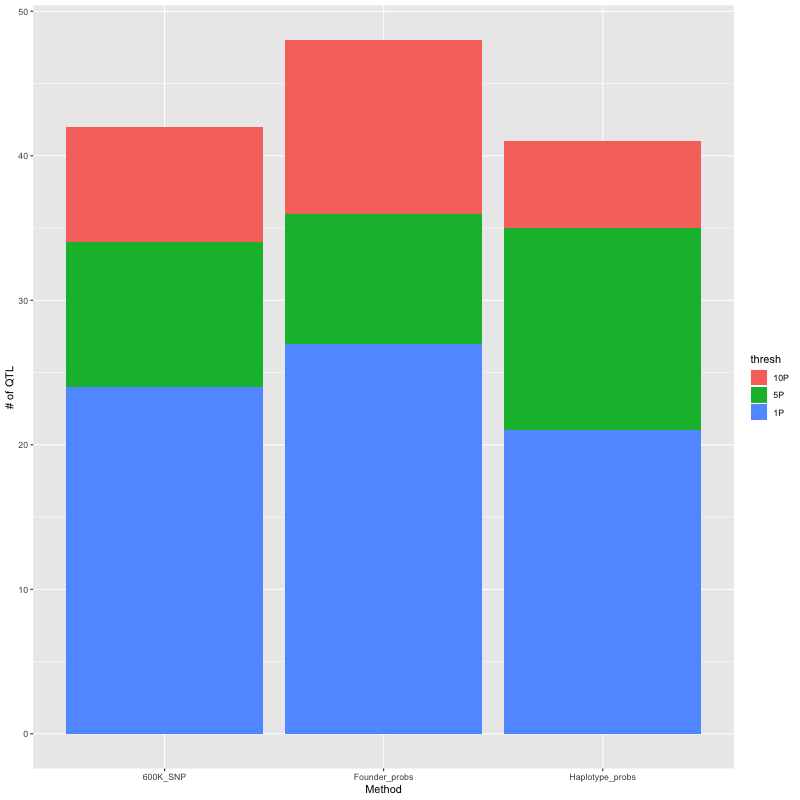
\includegraphics[width=\textwidth,height=14cm]{figures/threshold_by_method_counts.png}
\caption{\textbf{Total Number of Environment-QTL Found By Method By Significance Threshold} S: $GWAS_{SNP}$, F: $QTL_F$, H: $QTL_H$. Environment-specific QTL are QTL for a phenotype that were identified in one environment. QTL were called as found by multiple methods if their support intervals overlapped (see Methods).}
\label{fig:supfigure3}
\end{figure}

\begin{figure}[ht]
\centering
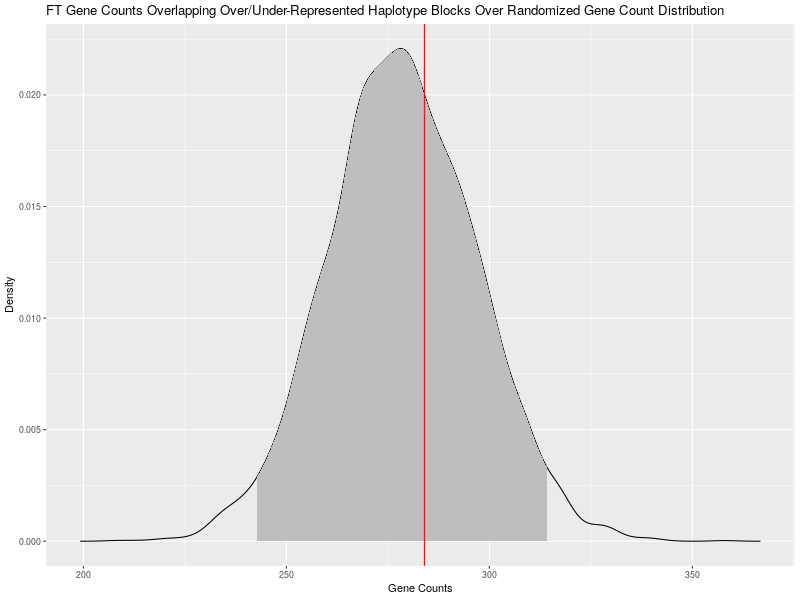
\includegraphics[width=\linewidth]{figures/ft_overlap_enrichment_density.png}
\caption{\textbf{Enrichment of Flowering Time Genes in $\rchi^2$ Peaks} Density plot of 1,000 permutations of number of 904 randomly selected genes that overlap with $\rchi^2$ peaks for over- or under-representation of haplotypes in the MAGIC population. Red line indicates the actual number (284) of FT genes from the list of 904 that overlapped with $\rchi^2$ peaks.}
\label{fig:supfigure4}
\end{figure}

%\blindtext
%\begin{figure*}[h!]
%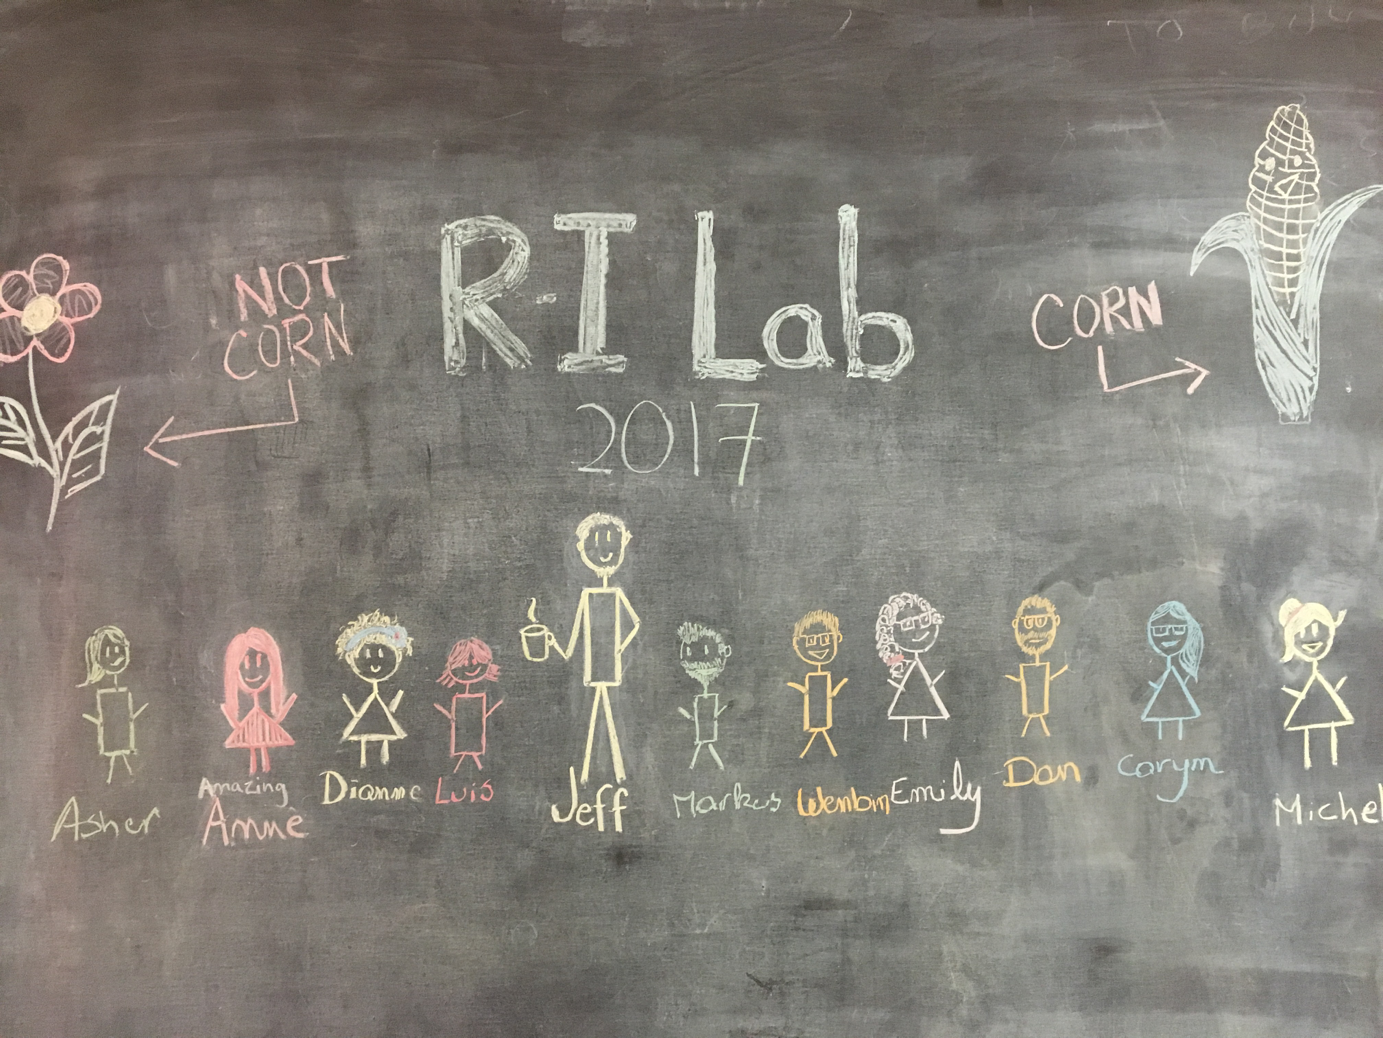
\includegraphics[width=.9\linewidth]{figures/lab_group.png}
%\caption{\textbf{Supplemental figure} Test test test}
%\label{fig:S1}
%\end{figure*}
\pagebreak


%\begin{table*}[htbp]
%\centering

%\caption{\bf Shrink a large table to fit the page}
%\begin{adjustbox}{totalheight=\textheight-2\baselineskip}
%\begin{tableminipage}{\textwidth}
%\begin{small}
%\begin{tabularx}{\textwidth}{sb}
%\hline
%Parameter & Description \\
%\hline
%\textbf{Adaptation} & \textbf{Trait related parameters} \\
%\hline
%Time to optimum & Generations until new optimum is reached \\
%Adaptation rate (haldane) & Adaptation rate until new optimum is reached. Calculated as $rate(h) = \frac{\frac{ln(x_2)}{sd_{x_{12}}}-\frac{ln(x_1)}{sd_{x_{12}}}}{t_2-t_1}$ \\
%Final genetic variance & Genetic variance in the final generation \\
%\textbf{Fixations} & \textbf{Mutations that fix after the optimum shift} \\
%\hline
%From new mutations (\#) & Sum of fixed mutations in the final population that were already segregating before  the optimum shift \\
%From standing variation (\#) & Sum of fixed mutations in the final population that arose after the optimum shift \\
%Max. effect size & Maximal effect size of all fixations \\
%Mean effect size & Mean effect size of all fixations \\
%Mean effect size of negative fixations & Mean effect size of negative mutations \\
%Mean effect size of positive fixations & Mean effect size of positive mutations \\
%Mean emergence time & Mean generation when a mutation arose that fixed in the last 0.1 N generations \\
%Mean fixation time & Mean generation in which a mutation fixed \\
%Min. effect size & Minimal effect size of all fixations \\
%Negative (\#) & Sum of fixed mutations with negative effects in the final population \\
%New/standing fixations & Ratio of mutations from new mutations vs. standing mutations  \\
%Proportion negative & Proportion of negative fixations from all mutations \\
%Positive (\#) & Sum of fixed mutations with positive effects in the final population \\
%SD of effect sizes & Standard deviation of effect sizes of all fixations \\
%SD of negative effect sizes & Standard deviation of effect sizes of negative fixations \\
%SD of positive effect sizes & Standard deviation of effect sizes of positive fixations \\
%Total (\#) & Sum of fixed mutations in the final population \\
%\textbf{Sweeps} & \textbf{Mutations that fix faster than 99\% of neutral fixations} \\
%\hline
%Hard sweeps (\#) & Sum of selective sweeps from new mutations \\
%Proportion of hard sweeps & Porportion of hard selective sweeps of all selective sweeps \\
%Proportion of sweeps from standing & Proportion of selective sweeps from stainding variation of all selection sweeps \\
%Sweeps (\#) & Sum of selective sweeps \\
%Sweeps from standing variation (\#) & Sum of selective sweeps from mutations that were already segregating before  the optimum shift \\
%Sweeps/fixations & Ratio of sweeps vs. fixations \\
%\textbf{Segregating sites} & \textbf{Mutations that segregate in the final generation} \\
%\hline
%Max. effect size & Maximal effect size of segregating sites \\
%Mean effect size & Mean effect size of segregating sites \\
%Mean effect size of negative sites & Mean effect size of segregating sites %with negative effects \\
%Mean effect size of positive sites & Mean effect size of segregating sites with positive effects \\
%Mean frequency of all sites & Mean allele frequency of segregating sites \\
%Mean frequency of negative sites & Mean allele frequency of segregating sites with negative effects \\
%Mean frequency of positive sites & Mean allele frequency of segregating sites with positive effects \\
%Min. effect size & Minimal effect size of segregating sites \\
%Negative (\#) & Sum of segregating sites with negative effect \\
%Positive (\#) & Sum of segregating sites with positive effect \\
%Proportion of negative sites & Proportion of segregating sites with negative effect of all segregating sites \\
%Standard deviation of effect sizes & Standard deviation of effect sizes of all segregating sites \\
%Total (\#) & Sum segregating sites in the final generation \\
%\hline

%\end{tabularx}
%  \label{tab:parameter_list}
%  \end{small}
%\end{tableminipage}

%\end{adjustbox}
%\end{table*}


\end{document}
